\selectlanguage{english}
\noindent{}GONÇALVES, J.F., 
RESENDE, M.G., 
TOSO, R.F., 
VIEIRA, S.R.R. \textbf{AN EXPERIMENTAL COMPARISON OF BIASED AND UNBIASED RANDOM-KEY GENETIC ALGORITHMS} Pesquisa Operacional. 34(2): 143-164. \url{http://dx.doi.org/10.1590/0101-7438.2014.034.02.0143}\bigskip{}

{
\renewcommand{\abstractname}{Abstract}
\begin{abstract}
\begin{spacing}{0.93}
Random key genetic algorithms are heuristic methods for solving combinatorial optimization problems.\allowbreak{} They represent solutions as vectors of randomly generated real numbers,\allowbreak{} the so-\allowbreak{}called random keys.\allowbreak{} A deterministic algorithm,\allowbreak{} called a decoder,\allowbreak{} takes as input a vector of random keys and associates with it a feasible solution of the combinatorial optimization problem for which an objective value or fitness can be computed.\allowbreak{} We compare three types of random-\allowbreak{}key genetic algorithms:\allowbreak{} the unbiased algorithm of Bean (\allowbreak{}1994)\allowbreak{}; the biased algorithm of Gonçalves and Resende (\allowbreak{}2010)\allowbreak{}; and a greedy version of Bean's algorithm on 12 instances from four types of covering problems:\allowbreak{} general-\allowbreak{}cost set covering,\allowbreak{} Steiner triple covering,\allowbreak{} general-\allowbreak{}cost set \textit{k} -\allowbreak{}covering,\allowbreak{} and unit-\allowbreak{}cost covering by pairs.\allowbreak{} Experiments are run to construct runtime distributions for 36 heuristic\fshyp{}instance pairs.\allowbreak{} For all pairs of heuristics,\allowbreak{} we compute probabilities that one heuristic is faster than the other on all 12 instances.\allowbreak{} The experiments show that,\allowbreak{} in 11 of the 12 instances,\allowbreak{} the greedy version of Bean's algorithm is faster than Bean's original method and that the biased variant is faster than both variants of Bean's algorithm.\allowbreak{}
\end{spacing}
\vspace*{1.9mm}
\fontsize{9}{10.8}\selectfont{\textit{Keywords:} genetic algorithm, biased random-\allowbreak{}key genetic algorithm, random keys, combinatorial optimization, heuristics, metaheuristics, experimental algorithms}
\end{abstract}
}

\vspace*{-1.6mm}
{\noindent\fontsize{9}{10.8}\selectfont{Received: 03/06/2014;
Accepted: 14/06/2014.}}
\begin{multicols}{2}
\section*{INTRODUCTION}
\par{}Genetic algorithms with random keys,\allowbreak{} or \textit{random-\allowbreak{}key genetic algorithms} (\allowbreak{}RKGA)\allowbreak{},\allowbreak{} were first introduced by \textsuperscript{Bean (\allowbreak{}1994)\allowbreak{}} for combinatorial optimization problems for which solutions can be represented as a permutation vector,\allowbreak{} e.\allowbreak{} g.\allowbreak{} sequencing and quadratic assignment.\allowbreak{} In a RKGA,\allowbreak{} chromosomes are represented as vectors of randomly generated real numbers in the interval [0,\allowbreak{} 1)\allowbreak{}.\allowbreak{} A deterministic algorithm,\allowbreak{} called a \textit{decoder},\allowbreak{} takes as input a solution vector and associates with it a feasible solution of the combinatorial optimization problem for which an objective value or \textit{fitness} can be computed.\allowbreak{} In a minimization (\allowbreak{}resp.\allowbreak{} maximization)\allowbreak{} problem,\allowbreak{} we say that solutions with smaller (\allowbreak{}resp.\allowbreak{} larger)\allowbreak{} objective function values are more fit than those with larger (\allowbreak{}resp.\allowbreak{} smaller)\allowbreak{} values.\allowbreak{}\par{}A RKGA evolves a population of random-\allowbreak{}key vectors over a number of iterations,\allowbreak{} called \textit{generations}.\allowbreak{} The initial population is made up of \textit{p} real \textit{n} -\allowbreak{}vectors of random keys.\allowbreak{} Each component of the solution vector is generated independently of each other at random in the real interval [0,\allowbreak{} 1)\allowbreak{}.\allowbreak{} After the fitness of each individual is computed by the decoder in generation \textit{k},\allowbreak{} the population is partitioned into two groups of individuals (\allowbreak{}see Fig.\allowbreak{} 1)\allowbreak{}:\allowbreak{} a small group of \textit{p\textsubscript{e} elite} individuals,\allowbreak{} i.\allowbreak{} e.\allowbreak{} those with the best fitness values,\allowbreak{} and the remaining set of \textit{p -\allowbreak{} p\textsubscript{e} non-\allowbreak{}elite} individuals.\allowbreak{} To evolve the population,\allowbreak{} a new generation of individuals must be produced.\allowbreak{} All elite individual of the population of generation \textit{k} are copied without modification to the population of generation \textit{k} +\allowbreak{} 1 (\allowbreak{}see Fig.\allowbreak{} 2)\allowbreak{}.\allowbreak{} Mutation,\allowbreak{} in genetic algorithms as well as in biology,\allowbreak{} is key for evolution of the population.\allowbreak{} RKGAs implement mutation by introducing \textit{mutants} into the population.\allowbreak{} A mutant is simply a vector of random keys generated in the same way as an element of the initial population.\allowbreak{} At each generation,\allowbreak{} a small number (\allowbreak{} \textit{p \textsubscript{m}})\allowbreak{} of mutants is introduced into the population (\allowbreak{}see Fig.\allowbreak{} 2)\allowbreak{}.\allowbreak{} With the \textit{p \textsubscript{e}} elite individuals and the \textit{p \textsubscript{m}} mutants accounted for in population \textit{k} +\allowbreak{} 1,\allowbreak{} \textit{p -\allowbreak{} p\textsubscript{e} -\allowbreak{} p \textsubscript{m}} additional individuals need to be produced to complete the \textit{p} individuals that make up the new population.\allowbreak{} This is done by producing \textit{p -\allowbreak{} p\textsubscript{e} -\allowbreak{} p \textsubscript{m}} offspring through the process of mating or crossover (\allowbreak{}see Fig.\allowbreak{} 3)\allowbreak{}.\allowbreak{}
\par
{
\centering{

\includegraphics[width=\maxwidth{0.5\textwidth}]{not-found.png}
}
\captionof{figure}{\textbf{Figure 1:} \textit{Population of \textit{p} solutions is partitioned into a smaller set of \textit{p\textsubscript{e}} elite (\allowbreak{}most fit)\allowbreak{} solutions and a larger set of \textit{p} $\allowbreak{\allowbreak{}\allowbreak{}}\allowbreak{}−$\allowbreak{\allowbreak{}\allowbreak{}}\allowbreak{} \textit{p\textsubscript{e}} non-\allowbreak{}elite (\allowbreak{}least fit)\allowbreak{} solutions.\allowbreak{}}} 
}
\par

\par
{
\centering{

\includegraphics[width=\maxwidth{0.5\textwidth}]{not-found.png}
}
\captionof{figure}{\textbf{Figure 2:} \textit{All \textit{p\textsubscript{e}} elite solutions from population \textit{k} are copied unchanged to population \textit{k} +\allowbreak{} 1 and \textit{p\textsubscript{m}} mutant solutions are generated in population \textit{k} +\allowbreak{} 1 as random-\allowbreak{}key vectors.\allowbreak{}}} 
}
\par

\par
{
\centering{

\includegraphics[width=\maxwidth{0.5\textwidth}]{not-found.png}
}
\captionof{figure}{\textbf{Figure 3:} \textit{To complete population \textit{k} +\allowbreak{} 1,\allowbreak{} p $\allowbreak{\allowbreak{}\allowbreak{}}\allowbreak{}−$\allowbreak{\allowbreak{}\allowbreak{}}\allowbreak{} \textit{p\textsubscript{e}} $\allowbreak{\allowbreak{}\allowbreak{}}\allowbreak{}−$\allowbreak{\allowbreak{}\allowbreak{}}\allowbreak{} \textit{p\textsubscript{m}} offspring are created by combining a parent selected at random from the elite set of population \textit{k} with a parent selected at random from the non-\allowbreak{}elite set of population \textit{k}.\allowbreak{} Parents can be selected for mating more than once per generation.\allowbreak{}}} 
}
\par
\par{}\textsuperscript{Bean (\allowbreak{}1994)\allowbreak{}} selects two parents at random from the entire population to implement mating in a RKGA and allows a parent to be selected more than once in a given generation.\allowbreak{} One parent is referred to as \textit{parent A} while the other is \textit{parent B}.\allowbreak{} A \textit{biased random-\allowbreak{}key genetic algorithm,\allowbreak{}} or BRKGA (\allowbreak{}\textsuperscript{Gonçalves \&\allowbreak{\allowbreak{}\allowbreak{}}\allowbreak{} Resende,\allowbreak{} 2011})\allowbreak{},\allowbreak{} differs from a RKGA in the way parents are selected for mating.\allowbreak{} In a BRKGA,\allowbreak{} each element is generated combining one element selected at random from the elite partition (\allowbreak{}this is \textit{parent A})\allowbreak{} in the current population and one from the non-\allowbreak{}elite partition (\allowbreak{}\textit{parent} B)\allowbreak{}.\allowbreak{} We say the selection is \textit{biased} since one parent is always an elite individual.\allowbreak{} Repetition in the selection of a mate is allowed and therefore an individual can produce more than one offspring in the same generation.\allowbreak{} \textit{Parameterized uniform crossover} (\allowbreak{}\textsuperscript{Spears \&\allowbreak{\allowbreak{}\allowbreak{}}\allowbreak{} DeJong,\allowbreak{} 1991})\allowbreak{} is used to implement mating in both RKGAs and BRKGAs.\allowbreak{} Let $\allowbreak{\allowbreak{}\allowbreak{}}\allowbreak{}ρ$\allowbreak{\allowbreak{}\allowbreak{}}\allowbreak{}A >0.\allowbreak{} 5 be the probability that an offspring inherits the vector component of parent A.\allowbreak{} Let \textit{n} denote the number of components in the solution vector of an individual.\allowbreak{} For \textit{i} = 1,\allowbreak{} .\allowbreak{}.\allowbreak{}.\allowbreak{},\allowbreak{} \textit{n},\allowbreak{} the \textit{i} -\allowbreak{}th component c(\allowbreak{}\textit{i})\allowbreak{} of the offspring vector \textit{c} takes on the value of the \textit{i} -\allowbreak{}th component \textit{a} (\allowbreak{}\textit{i})\allowbreak{} of parent \textit{A} with probability $\allowbreak{\allowbreak{}\allowbreak{}}\allowbreak{}ρ$\allowbreak{\allowbreak{}\allowbreak{}}\allowbreak{}\textit{A} and the value of the \textit{i} -\allowbreak{}th component \textit{b} (\allowbreak{}\textit{i})\allowbreak{} of parent \textit{B} with probability 1 -\allowbreak{}\textit{$\allowbreak{\allowbreak{}\allowbreak{}}\allowbreak{}ρ$\allowbreak{\allowbreak{}\allowbreak{}}\allowbreak{}A}.\allowbreak{} In this paper,\allowbreak{} we also consider a slight variation of Bean's algorithm,\allowbreak{} which we call RKGA*\allowbreak{},\allowbreak{} where once two parents are selected for mating,\allowbreak{} the best fit of the two is called parent \textit{A} while the other is parent \textit{B}.\allowbreak{} Box 1:\allowbreak{}\par{}When the next population is complete,\allowbreak{} i.\allowbreak{} e.\allowbreak{} when it has \textit{p} individuals,\allowbreak{} fitness values are computed by the decoder for all of the newly created random-\allowbreak{}key vectors and the population is partitioned into elite and non-\allowbreak{}elite individuals to start a new generation.\allowbreak{} Figure 4 shows a flow diagram of the BRKGA framework with a clear separation between the problem dependent and problem independent components of the method.\allowbreak{}
\par
{
\centering{

\includegraphics[width=\maxwidth{0.5\textwidth}]{not-found.png}
}
\captionof{figure}{\textbf{Figure 4:} \textit{Flowchart of random-\allowbreak{}key genetic algorithm with problem independent and problem dependent components.\allowbreak{}}} 
}
\par
\par{}Random-\allowbreak{}key genetic algorithms search the solution space of the combinatorial optimization problem indirectly by exploring the continuous \textit{n} -\allowbreak{}dimensional hypercube,\allowbreak{} using the decoder to map solutions in the hypercube to solutions in the solution space of the combinatorial optimization problem where the fitness is evaluated.\allowbreak{}\par{}As aforementioned,\allowbreak{} the role of mutants is to help the algorithm escape from local optima.\allowbreak{} An escape occurs when a locally-\allowbreak{}optimal elite solution is combined with a mutant and the resulting offspring is better fit than both parents.\allowbreak{} Another way to avoid getting stuck in local optima is to embed the random-\allowbreak{}key genetic algorithm in a multi-\allowbreak{}start strategy.\allowbreak{} After \textit{i \textsubscript{r}} > 0 generations without improvement in the fitness of the best solution,\allowbreak{} the best overall solution is tentatively updated with the best fit solution in the population,\allowbreak{} the population is discarded and the algorithm is restarted.\allowbreak{}\par{}To describe a random-\allowbreak{}key genetic algorithm for a specific combinatorial optimization problem,\allowbreak{} one needs only to show how solutions are encoded as vectors of random keys and how these vectors are decoded to feasible solutions of the optimization problem.\allowbreak{} In the next section,\allowbreak{} we describe random-\allowbreak{}key genetic algorithms for the four set covering problems problems considered in this paper.\allowbreak{}\par{}The paper is organized as follows.\allowbreak{} In Section 2 we describe the four covering problems and in Section 3 we propose random-\allowbreak{}key genetic algorithms for each problem.\allowbreak{} Experimental results comparing implementations of RKGA,\allowbreak{} RKGA*\allowbreak{},\allowbreak{} and BRKGA for each of the four covering problems are presented in Section 4.\allowbreak{} We make concluding remarks in Section 5.\allowbreak{} 
\section*{FOUR SET COVERING PROBLEMS}
\par{}In this section,\allowbreak{} we define four set covering problems and propose random-\allowbreak{}key genetic algorithms for each.\allowbreak{}\subsection*{2.\allowbreak{}1 General-\allowbreak{}cost set covering}
\par{}Given \textit{n} finite sets \textit{P \textsubscript{1}},\allowbreak{} \textit{P \textsubscript{2}},\allowbreak{} .\allowbreak{}.\allowbreak{}.\allowbreak{},\allowbreak{} \textit{P \textsubscript{n}},\allowbreak{} let sets \textit{I } and \textit{J} be defined as \textit{I} = $\allowbreak{\allowbreak{}\allowbreak{}}\allowbreak{}∪$\allowbreak{\allowbreak{}\allowbreak{}}\allowbreak{}\textit{\textsuperscript{n} j P \textsubscript{j}} =\{\allowbreak{}\allowbreak{}1,\allowbreak{}2,\allowbreak{} .\allowbreak{}.\allowbreak{}.\allowbreak{},\allowbreak{} \textit{m} \}\allowbreak{} and \textit{J} =\{\allowbreak{}\allowbreak{}1,\allowbreak{} .\allowbreak{}.\allowbreak{}.\allowbreak{},\allowbreak{} \textit{n} \}\allowbreak{}.\allowbreak{} Associate a cost \textit{c \textsubscript{j}} > 0 with each element \textit{j} $\allowbreak{\allowbreak{}\allowbreak{}}\allowbreak{}∈$\allowbreak{\allowbreak{}\allowbreak{}}\allowbreak{}\textit{ J }.\allowbreak{} A subset \textit{J} *\allowbreak{} $\allowbreak{\allowbreak{}\allowbreak{}}\allowbreak{}⊆$\allowbreak{\allowbreak{}\allowbreak{}}\allowbreak{} \textit{J} is called a \textit{cover} if $\allowbreak{\allowbreak{}\allowbreak{}}\allowbreak{}∪$\allowbreak{\allowbreak{}\allowbreak{}}\allowbreak{}\textit{\textsubscript{j$\allowbreak{\allowbreak{}\allowbreak{}}\allowbreak{}∈$\allowbreak{\allowbreak{}\allowbreak{}}\allowbreak{}J} *\allowbreak{} P \textsubscript{j} = I}.\allowbreak{} The cost of the cover is $\allowbreak{\allowbreak{}\allowbreak{}}\allowbreak{}Σ$\allowbreak{\allowbreak{}\allowbreak{}}\allowbreak{} \textit{\textsubscript{j$\allowbreak{\allowbreak{}\allowbreak{}}\allowbreak{}∈$\allowbreak{\allowbreak{}\allowbreak{}}\allowbreak{}J*\allowbreak{}} c \textsubscript{j}}.\allowbreak{} The \textit{set covering problem } is to find a minimum cost cover.\allowbreak{} Let \textit{A} be the binary \textit{m} $\allowbreak{\allowbreak{}\allowbreak{}}\allowbreak{}×$\allowbreak{\allowbreak{}\allowbreak{}}\allowbreak{} \textit{n} matrix such that \textit{A \textsubscript{i,\allowbreak{} j}} = 1 if and only if \textit{i} $\allowbreak{\allowbreak{}\allowbreak{}}\allowbreak{}∈$\allowbreak{\allowbreak{}\allowbreak{}}\allowbreak{}\textit{P \textsubscript{j}}.\allowbreak{} An integer programming formulation for set covering is\par{}min \{\allowbreak{}\allowbreak{}\textit{cx :\allowbreak{} Ax} $\allowbreak{\allowbreak{}\allowbreak{}}\allowbreak{}≥$\allowbreak{\allowbreak{}\allowbreak{}}\allowbreak{}\textit{ e \textsubscript{m},\allowbreak{} x} $\allowbreak{\allowbreak{}\allowbreak{}}\allowbreak{}∈$\allowbreak{\allowbreak{}\allowbreak{}}\allowbreak{}\{\allowbreak{}\allowbreak{}0,\allowbreak{}1\}\allowbreak{}\textit{\textsuperscript{n}} \}\allowbreak{},\allowbreak{}\par{}where \textit{e \textsubscript{m}} denotes a vector of \textit{m} ones and \textit{x} is a binary \textit{n} -\allowbreak{}vector such that \textit{x \textsubscript{j}} =1 if and only if \textit{j} $\allowbreak{\allowbreak{}\allowbreak{}}\allowbreak{}∈$\allowbreak{\allowbreak{}\allowbreak{}}\allowbreak{} \textit{J*\allowbreak{}}.\allowbreak{} The set covering problem has many applications (\allowbreak{}\textsuperscript{Vemuganti,\allowbreak{} 1998})\allowbreak{} and is NP-\allowbreak{}hard (\allowbreak{}\textsuperscript{Garey \&\allowbreak{\allowbreak{}\allowbreak{}}\allowbreak{} Johnson,\allowbreak{} 1979})\allowbreak{}.\allowbreak{}
\subsection*{2.\allowbreak{}2 Unit-\allowbreak{}cost set covering}
\par{}A special case of set covering is where \textit{c \textsubscript{j }} = 1,\allowbreak{} for all \textit{j} $\allowbreak{\allowbreak{}\allowbreak{}}\allowbreak{}∈$\allowbreak{\allowbreak{}\allowbreak{}}\allowbreak{} \textit{J}.\allowbreak{} This problem is called the unitcost set covering problem and its objective can be thought of as finding a cover of minimum cardinality.\allowbreak{}
\subsection*{2.\allowbreak{}3 General-\allowbreak{}cost set k-\allowbreak{}covering}
\par{}The \textit{set k-\allowbreak{}covering problem} is a generalization of the set covering problem,\allowbreak{} in which each object \textit{i} $\allowbreak{\allowbreak{}\allowbreak{}}\allowbreak{}∈$\allowbreak{\allowbreak{}\allowbreak{}}\allowbreak{} \textit{I} must be covered by at least \textit{k} elements of \{\allowbreak{}\allowbreak{}\textit{P \textsubscript{1}},\allowbreak{} .\allowbreak{}.\allowbreak{}.\allowbreak{},\allowbreak{} \textit{P \textsubscript{n}} \}\allowbreak{}.\allowbreak{} As before,\allowbreak{} let \textit{A} be the binary \textit{m} $\allowbreak{\allowbreak{}\allowbreak{}}\allowbreak{}×$\allowbreak{\allowbreak{}\allowbreak{}}\allowbreak{}\textit{ n} matrix such that \textit{A \textsubscript{i,\allowbreak{} j}} = 1 if and only if \textit{i} $\allowbreak{\allowbreak{}\allowbreak{}}\allowbreak{}∈$\allowbreak{\allowbreak{}\allowbreak{}}\allowbreak{}\textit{P \textsubscript{j}}.\allowbreak{} An integer programming formulation for set \textit{k} -\allowbreak{}covering is\par{}min \{\allowbreak{}\allowbreak{}\textit{cx :\allowbreak{} Ax} $\allowbreak{\allowbreak{}\allowbreak{}}\allowbreak{}≥$\allowbreak{\allowbreak{}\allowbreak{}}\allowbreak{}\textit{ km,\allowbreak{} x} $\allowbreak{\allowbreak{}\allowbreak{}}\allowbreak{}∈$\allowbreak{\allowbreak{}\allowbreak{}}\allowbreak{}\{\allowbreak{}\allowbreak{}0,\allowbreak{}1\}\allowbreak{}\textit{\textsuperscript{n}} \}\allowbreak{},\allowbreak{}\par{}where \textit{k \textsubscript{m}} denotes an \textit{m} -\allowbreak{}vector of all \textit{k} s.\allowbreak{} For example,\allowbreak{} \textit{k \textsubscript{4}} = (\allowbreak{}\textit{k,\allowbreak{} k,\allowbreak{} k,\allowbreak{} k})\allowbreak{}\textsuperscript{T}.\allowbreak{}\par{}Note that the set covering problem (\allowbreak{}Subsection 2.\allowbreak{} 1)\allowbreak{} as well as the unit-\allowbreak{}cost set covering problem (\allowbreak{}Subsection 2.\allowbreak{} 2)\allowbreak{} are special cases of set \textit{k} -\allowbreak{}covering.\allowbreak{} In both,\allowbreak{} \textit{k} = 1 and,\allowbreak{} furthermore,\allowbreak{} in unit-\allowbreak{}cost set covering \textit{c \textsubscript{j}} = 1 for all \textit{j} $\allowbreak{\allowbreak{}\allowbreak{}}\allowbreak{}∈$\allowbreak{\allowbreak{}\allowbreak{}}\allowbreak{}\textit{J}.\allowbreak{}
\subsection*{2.\allowbreak{}4 Covering by pairs}
\par{}Let \textit{I} = \{\allowbreak{}\allowbreak{}1,\allowbreak{} 2,\allowbreak{} .\allowbreak{}.\allowbreak{}.\allowbreak{},\allowbreak{} \textit{m} \}\allowbreak{},\allowbreak{} \textit{J} = \{\allowbreak{}\allowbreak{}1,\allowbreak{} 2,\allowbreak{} .\allowbreak{}.\allowbreak{}.\allowbreak{},\allowbreak{} \textit{n} \}\allowbreak{},\allowbreak{} and associate with each element of \textit{j} $\allowbreak{\allowbreak{}\allowbreak{}}\allowbreak{}∈$\allowbreak{\allowbreak{}\allowbreak{}}\allowbreak{} \textit{J} acost \textit{c \textsubscript{j}} > 0.\allowbreak{} For every pair \{\allowbreak{}\allowbreak{}\textit{j,\allowbreak{} k} \}\allowbreak{} $\allowbreak{\allowbreak{}\allowbreak{}}\allowbreak{}∈$\allowbreak{\allowbreak{}\allowbreak{}}\allowbreak{} \textit{J} $\allowbreak{\allowbreak{}\allowbreak{}}\allowbreak{}×$\allowbreak{\allowbreak{}\allowbreak{}}\allowbreak{}\textit{ J},\allowbreak{} with \textit{j} $\allowbreak{\allowbreak{}\allowbreak{}}\allowbreak{}≠$\allowbreak{\allowbreak{}\allowbreak{}}\allowbreak{}\textit{ k},\allowbreak{} let $\allowbreak{\allowbreak{}\allowbreak{}}\allowbreak{}π$\allowbreak{\allowbreak{}\allowbreak{}}\allowbreak{} (\allowbreak{}\textit{j,\allowbreak{} k})\allowbreak{} be the subset of elements in \textit{I} covered by pair \{\allowbreak{}\allowbreak{}\textit{j,\allowbreak{} k} \}\allowbreak{}.\allowbreak{} A subset \textit{J} *\allowbreak{} $\allowbreak{\allowbreak{}\allowbreak{}}\allowbreak{}⊆$\allowbreak{\allowbreak{}\allowbreak{}}\allowbreak{} \textit{J} is a cover by pairs if\begin{center}
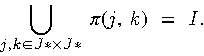
\includegraphics[width=\maxwidth{0.5\textwidth}]{mathml/math1.pdf}
\end{center}
\par{}The cost of \textit{J} *\allowbreak{} is $\allowbreak{\allowbreak{}\allowbreak{}}\allowbreak{}Σ$\allowbreak{\allowbreak{}\allowbreak{}}\allowbreak{}\textit{\textsubscript{j$\allowbreak{\allowbreak{}\allowbreak{}}\allowbreak{}∈$\allowbreak{\allowbreak{}\allowbreak{}}\allowbreak{}J*\allowbreak{}} c \textsubscript{j}}.\allowbreak{} The \textit{set covering by pairs problem } is to find a minimum cost cover by pairs.\allowbreak{}\par{}For all \textit{j} $\allowbreak{\allowbreak{}\allowbreak{}}\allowbreak{}∈$\allowbreak{\allowbreak{}\allowbreak{}}\allowbreak{} \textit{J},\allowbreak{} let \textit{x \textsubscript{j}} be a binary variable such that \textit{x \textsubscript{j}} = 1 if and only if \textit{j} $\allowbreak{\allowbreak{}\allowbreak{}}\allowbreak{}∈$\allowbreak{\allowbreak{}\allowbreak{}}\allowbreak{} \textit{J} *\allowbreak{}.\allowbreak{} For every pair \{\allowbreak{}\allowbreak{}\textit{j,\allowbreak{} k} \}\allowbreak{} $\allowbreak{\allowbreak{}\allowbreak{}}\allowbreak{}∈$\allowbreak{\allowbreak{}\allowbreak{}}\allowbreak{} \textit{J} $\allowbreak{\allowbreak{}\allowbreak{}}\allowbreak{}×$\allowbreak{\allowbreak{}\allowbreak{}}\allowbreak{} \textit{J} with \textit{j} < \textit{k},\allowbreak{} let the continuous variable \textit{y \textsubscript{jk}} be such that \textit{y \textsubscript{jk}} $\allowbreak{\allowbreak{}\allowbreak{}}\allowbreak{}≤$\allowbreak{\allowbreak{}\allowbreak{}}\allowbreak{}\textit{ x \textsubscript{j}} and \textit{y \textsubscript{jk}} $\allowbreak{\allowbreak{}\allowbreak{}}\allowbreak{}≤$\allowbreak{\allowbreak{}\allowbreak{}}\allowbreak{}\textit{ x \textsubscript{k}}.\allowbreak{} Therefore,\allowbreak{} if \textit{y \textsubscript{jk}} > 0 then \textit{x \textsubscript{j} = x \textsubscript{k}} = 1.\allowbreak{} Let $\allowbreak{\allowbreak{}\allowbreak{}}\allowbreak{}π$\allowbreak{\allowbreak{}\allowbreak{}}\allowbreak{}\textsuperscript{-\allowbreak{}1}(\allowbreak{}\textit{i})\allowbreak{} denote the set of pairs \{\allowbreak{}\allowbreak{}\textit{j,\allowbreak{} k} \}\allowbreak{} $\allowbreak{\allowbreak{}\allowbreak{}}\allowbreak{}∈$\allowbreak{\allowbreak{}\allowbreak{}}\allowbreak{} \textit{J} $\allowbreak{\allowbreak{}\allowbreak{}}\allowbreak{}×$\allowbreak{\allowbreak{}\allowbreak{}}\allowbreak{}\textit{ J} that cover \textit{i} $\allowbreak{\allowbreak{}\allowbreak{}}\allowbreak{}∈$\allowbreak{\allowbreak{}\allowbreak{}}\allowbreak{}\textit{I}.\allowbreak{} An integer programming formulation for the covering by pairs problem is\begin{center}
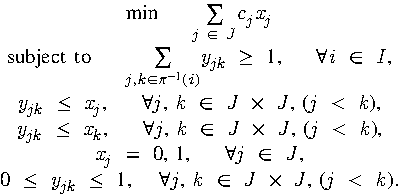
\includegraphics[width=\maxwidth{0.5\textwidth}]{mathml/math2.pdf}
\end{center}


\section*{RANDOM-\allowbreak{}KEY GENETIC ALGORITHMS FOR COVERING}
\par{}Biased random-\allowbreak{}key genetic algorithms for set covering have been proposed by \textsuperscript{Resende et al.\allowbreak{} (\allowbreak{}2012)\allowbreak{}},\allowbreak{} \textsuperscript{Breslau et al.\allowbreak{} (\allowbreak{}2011)\allowbreak{}},\allowbreak{} and \textsuperscript{Pessoa et al.\allowbreak{} (\allowbreak{}2011)\allowbreak{}}.\allowbreak{} These include a BRKGA for the Steiner triple covering problem,\allowbreak{} a unit-\allowbreak{}cost set covering problem (\allowbreak{}\textsuperscript{Resende et al.\allowbreak{} ,\allowbreak{} 2012})\allowbreak{},\allowbreak{} BRKGA heuristics for the set covering and set \textit{k} -\allowbreak{}covering problems (\allowbreak{}\textsuperscript{Pessoa et al.\allowbreak{},\allowbreak{} 2011})\allowbreak{},\allowbreak{} and a BRKGA for set covering by pairs (\allowbreak{}\textsuperscript{Breslau et al.\allowbreak{} ,\allowbreak{} 2011})\allowbreak{}.\allowbreak{} We review these heuristics in the remainder of this section.\allowbreak{}\par{}The random-\allowbreak{}key genetic algorithms for the set covering problems of Section 2 that we describe in this section all encode solutions as a |\textit{J} |-\allowbreak{}vector X of random keys.\allowbreak{} The \textit{j} -\allowbreak{}th key X\textit{\textsubscript{j}} corresponds to the \textit{j} -\allowbreak{}th element of set \textit{J}.\allowbreak{}\par{}Decoding is similar for all four covering problems.\allowbreak{} The decoding scheme has three steps.\allowbreak{} In step 1,\allowbreak{} a tentative cover solution \textit{J} *\allowbreak{} is constructed by placing in \textit{J} *\allowbreak{} all elements \textit{j} $\allowbreak{\allowbreak{}\allowbreak{}}\allowbreak{}∈$\allowbreak{\allowbreak{}\allowbreak{}}\allowbreak{}\textit{J} for which X\textit{\textsubscript{j}} > 1\fshyp{}2.\allowbreak{} If \textit{J} *\allowbreak{} is a feasible cover,\allowbreak{} then step 2 is skipped.\allowbreak{} Otherwise,\allowbreak{} in step 2,\allowbreak{} a greedy algorithm is used to construct a valid cover starting from \textit{J} *\allowbreak{}.\allowbreak{} Later in this section,\allowbreak{} we describe these greedy algorithms.\allowbreak{} Finally,\allowbreak{} in step 3,\allowbreak{} a local improvement procedure is applied to the cover.\allowbreak{} Later in this section,\allowbreak{} we describe the different local improvement procedures.\allowbreak{}\par{}The decoder not only returns the cover \textit{J} *\allowbreak{} but also modifies the vector of random keys \textit{X} such that it decodes directly into \textit{J} *\allowbreak{} with the application of only the first phase of the decoder.\allowbreak{} To do this we reset X as follows:\allowbreak{}\begin{center}
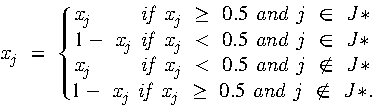
\includegraphics[width=\maxwidth{0.5\textwidth}]{mathml/math3.pdf}
\end{center}
\subsection*{Greedy algorithms}
\par{}We use two greedy algorithms.\allowbreak{} The first is for set \textit{k} -\allowbreak{}covering and its special cases,\allowbreak{} set covering and unit-\allowbreak{}cost set covering.\allowbreak{} The second one is for covering by pairs.\allowbreak{}\subsection*{3.\allowbreak{}1.\allowbreak{}1 Greedy algorithm for set k-\allowbreak{}covering}
\par{}A greedy algorithm for set covering (\allowbreak{}Johnson,\allowbreak{} 1974)\allowbreak{} starts from the partial cover \textit{J} *\allowbreak{} defined by \textit{X}.\allowbreak{} This greedy algorithm proceeds as follows.\allowbreak{} While \textit{J} *\allowbreak{} is not a valid cover,\allowbreak{} add to \textit{J} *\allowbreak{} the smallest index \textit{j} $\allowbreak{\allowbreak{}\allowbreak{}}\allowbreak{}∈$\allowbreak{\allowbreak{}\allowbreak{}}\allowbreak{} \textit{J} SCIELO\_\allowbreak{\allowbreak{}\allowbreak{}}\allowbreak{}BSHYP \textit{J} *\allowbreak{} for which the inclusion of \textit{j} in \textit{J} *\allowbreak{} corresponds to the minimum ratio $\allowbreak{\allowbreak{}\allowbreak{}}\allowbreak{}π$\allowbreak{\allowbreak{}\allowbreak{}}\allowbreak{}\textit{\textsubscript{j }} of cost \textit{c \textsubscript{j}} to number of yet-\allowbreak{}uncovered elements of \textit{I} that become covered with the inclusion of \textit{j} in \textit{J} *\allowbreak{} .\allowbreak{} For the special case of unit-\allowbreak{}cost set covering,\allowbreak{} this reduces to adding the smallest index \textit{j} $\allowbreak{\allowbreak{}\allowbreak{}}\allowbreak{}∈$\allowbreak{\allowbreak{}\allowbreak{}}\allowbreak{} \textit{J} SCIELO\_\allowbreak{\allowbreak{}\allowbreak{}}\allowbreak{}BSHYP \textit{J} *\allowbreak{} for which the inclusion of \textit{j} in \textit{J} *\allowbreak{} maximizes the number $\allowbreak{\allowbreak{}\allowbreak{}}\allowbreak{}π$\allowbreak{\allowbreak{}\allowbreak{}}\allowbreak{} \textit{j} of yet-\allowbreak{}uncovered elements of \textit{I} that become covered with the inclusion of \textit{j} in \textit{J} *\allowbreak{} .\allowbreak{} In this iterative process,\allowbreak{} we use a binary heap to store the $\allowbreak{\allowbreak{}\allowbreak{}}\allowbreak{}π$\allowbreak{\allowbreak{}\allowbreak{}}\allowbreak{}\textit{\textsubscript{j }} values of unused columns,\allowbreak{} allowing us to retrieve a column \textit{j} with largest $\allowbreak{\allowbreak{}\allowbreak{}}\allowbreak{}π$\allowbreak{\allowbreak{}\allowbreak{}}\allowbreak{}\textit{\textsubscript{j }} value in \textit{O} (\allowbreak{}log \textit{m})\allowbreak{}-\allowbreak{}time and update the $\allowbreak{\allowbreak{}\allowbreak{}}\allowbreak{}π$\allowbreak{\allowbreak{}\allowbreak{}}\allowbreak{} values of the remaining columns in \textit{O} (\allowbreak{}log \textit{n})\allowbreak{}-\allowbreak{}time after column \textit{j} is added to the solution.\allowbreak{}
\subsection*{Greedy algorithm for unit-\allowbreak{}cost covering by pairs}
\par{}A greedy algorithm for unit-\allowbreak{}cost covering by pairs is proposed in \textsuperscript{Breslau et al.\allowbreak{} (\allowbreak{}2011)\allowbreak{}}.\allowbreak{} It starts with set \textit{J} *\allowbreak{} defined by \textit{X}.\allowbreak{} Then,\allowbreak{} as long as \textit{J} *\allowbreak{} is not a valid cover,\allowbreak{} find an element \textit{j} $\allowbreak{\allowbreak{}\allowbreak{}}\allowbreak{}∈$\allowbreak{\allowbreak{}\allowbreak{}}\allowbreak{} \textit{J} SCIELO\_\allowbreak{\allowbreak{}\allowbreak{}}\allowbreak{}BSHYP \textit{J} *\allowbreak{} such that \textit{J} *\allowbreak{} $\allowbreak{\allowbreak{}\allowbreak{}}\allowbreak{}∪$\allowbreak{\allowbreak{}\allowbreak{}}\allowbreak{}\{\allowbreak{}\allowbreak{} \textit{f} \}\allowbreak{} covers a maximum number of yet-\allowbreak{}uncovered elements of \textit{I}.\allowbreak{} Ties are broken by the index of element \textit{j} .\allowbreak{} If the number of yet-\allowbreak{}uncovered elements of \textit{I} that become covered is at least one,\allowbreak{} add \textit{j} to \textit{J} *\allowbreak{} .\allowbreak{} Otherwise,\allowbreak{} find a pair of \{\allowbreak{}\allowbreak{}\textit{j \textsubscript{1}},\allowbreak{} \textit{j \textsubscript{2}} \}\allowbreak{}$\allowbreak{\allowbreak{}\allowbreak{}}\allowbreak{}⊆$\allowbreak{\allowbreak{}\allowbreak{}}\allowbreak{} \textit{J} SCIELO\_\allowbreak{\allowbreak{}\allowbreak{}}\allowbreak{}BSHYP\textit{J} *\allowbreak{} such that \textit{J} *\allowbreak{} $\allowbreak{\allowbreak{}\allowbreak{}}\allowbreak{}∪$\allowbreak{\allowbreak{}\allowbreak{}}\allowbreak{}\{\allowbreak{}\allowbreak{}\textit{j \textsubscript{1}} \}\allowbreak{}$\allowbreak{\allowbreak{}\allowbreak{}}\allowbreak{}∪$\allowbreak{\allowbreak{}\allowbreak{}}\allowbreak{}\{\allowbreak{}\allowbreak{}\textit{j \textsubscript{2}} \}\allowbreak{} covers a maximum number of yet-\allowbreak{}uncovered elements in \textit{I}.\allowbreak{} Ties are broken first by the index of \textit{j \textsubscript{1}} ,\allowbreak{}then by the index of \textit{j \textsubscript{2}} .\allowbreak{} If such a pair does not exist,\allowbreak{} then the problem is infeasible.\allowbreak{} Otherwise,\allowbreak{} add \textit{j \textsubscript{1}} and \textit{j \textsubscript{2}} to \textit{J} *\allowbreak{} .\allowbreak{}

\subsection*{Local improvement procedures}
\par{}Given a cover \textit{J} *\allowbreak{},\allowbreak{} the local improvement procedure attempts to make elementary modifications to the cover with the objective of reducing its cost.\allowbreak{} We use two types of local improvement procedures:\allowbreak{} \textit{greedy uncover} and \textit{1-\allowbreak{}opt}.\allowbreak{} In the decoder for set \textit{k} -\allowbreak{}covering we apply greedy uncover,\allowbreak{} followed by 1-\allowbreak{}opt,\allowbreak{} followed by greedy uncover if necessary.\allowbreak{} In the special case of unit-\allowbreak{}cost set covering only greedy uncover is used.\allowbreak{} The decoder implemented for set covering by pairs does not make use of any local improvement procedure.\allowbreak{} Instead,\allowbreak{} greedy uncover is applied to each elite solution after the iterations of the genetic algorithm end.\allowbreak{} In the experiments described in Section 4,\allowbreak{} this local improvement is not activated.\allowbreak{}\subsection*{Greedy uncover}
\par{}Given a cover \textit{J} *\allowbreak{},\allowbreak{} \textit{greedy uncover} attempts to remove superfluous elements of \textit{J} *\allowbreak{},\allowbreak{} i.\allowbreak{} e.\allowbreak{} elements \textit{j} $\allowbreak{\allowbreak{}\allowbreak{}}\allowbreak{}∈$\allowbreak{\allowbreak{}\allowbreak{}}\allowbreak{} \textit{J} *\allowbreak{} such that \textit{J} *\allowbreak{} SCIELO\_\allowbreak{\allowbreak{}\allowbreak{}}\allowbreak{}BSHYP\{\allowbreak{}\allowbreak{}\textit{j} \}\allowbreak{} is a cover.\allowbreak{} This is done by scanning the elements \textit{j} $\allowbreak{\allowbreak{}\allowbreak{}}\allowbreak{}∈$\allowbreak{\allowbreak{}\allowbreak{}}\allowbreak{} \textit{J} *\allowbreak{} in decreasing order of cost \textit{c \textsubscript{j}},\allowbreak{} removing those elements that are superfluous.\allowbreak{}
\subsection*{1-\allowbreak{}Opt}
\par{}Given a cover \textit{J} *\allowbreak{},\allowbreak{} \textit{1-\allowbreak{}Opt} attempts to find an element \textit{j} $\allowbreak{\allowbreak{}\allowbreak{}}\allowbreak{}∈$\allowbreak{\allowbreak{}\allowbreak{}}\allowbreak{} \textit{J} *\allowbreak{} and another element \textit{i} $\allowbreak{\allowbreak{}\allowbreak{}}\allowbreak{}∉$\allowbreak{\allowbreak{}\allowbreak{}}\allowbreak{} \textit{J} *\allowbreak{} such that \textit{c \textsubscript{i}} < \textit{c \textsubscript{j}} and \textit{J} *\allowbreak{} SCIELO\_\allowbreak{\allowbreak{}\allowbreak{}}\allowbreak{}BSHYP\{\allowbreak{}\allowbreak{}\textit{j} \}\allowbreak{} $\allowbreak{\allowbreak{}\allowbreak{}}\allowbreak{}∪$\allowbreak{\allowbreak{}\allowbreak{}}\allowbreak{} \{\allowbreak{}\allowbreak{}\textit{i} \}\allowbreak{} is a cover.\allowbreak{} If such a pair is found,\allowbreak{} \textit{i} replaces \textit{j} in \textit{J} *\allowbreak{} .\allowbreak{} This is done by scanning the elements \textit{j} $\allowbreak{\allowbreak{}\allowbreak{}}\allowbreak{}∈$\allowbreak{\allowbreak{}\allowbreak{}}\allowbreak{} \textit{J} *\allowbreak{} in decreasing order of cost \textit{c \textsubscript{j}} ,\allowbreak{} searching for an element \textit{i} $\allowbreak{\allowbreak{}\allowbreak{}}\allowbreak{}∉$\allowbreak{\allowbreak{}\allowbreak{}}\allowbreak{}\textit{J} *\allowbreak{} that covers all elements of \textit{I} left uncovered with the removal of each \textit{j} $\allowbreak{\allowbreak{}\allowbreak{}}\allowbreak{}∈$\allowbreak{\allowbreak{}\allowbreak{}}\allowbreak{} \textit{J} *\allowbreak{} .\allowbreak{}


\section*{COMPUTATIONAL EXPERIMENTS}
\par{}We report in this section computational results with the two variants of random-\allowbreak{}key genetic algorithms (\allowbreak{}the biased variant -\allowbreak{} BRKGA -\allowbreak{} and Bean's unbiased variant -\allowbreak{} RKGA)\allowbreak{} of Section 1 as well as a variant of Bean's algorithm which we shall refer to as RKGA*\allowbreak{}.\allowbreak{} Like Bean's RKGA,\allowbreak{} RKGA*\allowbreak{} selects both parents at random from the entire population.\allowbreak{} This is unlike a BRKGA,\allowbreak{} where one parent is always selected from the elite partition of the population and the other from the non-\allowbreak{}elite partition.\allowbreak{} Unlike Bean's algorithm,\allowbreak{} a RKGA*\allowbreak{} assigns the best fit of both parents as \textit{parent A} and the other as \textit{parent B} for crossover.\allowbreak{} Ties are broken by rank in the sorted population.\allowbreak{} RKGA assigns the selected parents to the roles of \textit{parent A} and \textit{parent B} at random.\allowbreak{}\par{}Our goal in these experiments is to compare these three types of heuristics on different problem instances and show that the BRKGA is the most effective of the three.\allowbreak{}\par{}In the experiments,\allowbreak{} we consider four problem types:\allowbreak{} general-\allowbreak{}cost set covering,\allowbreak{} Steiner triple (\allowbreak{}unit-\allowbreak{}cost)\allowbreak{} covering,\allowbreak{} general-\allowbreak{}cost set \textit{k} -\allowbreak{}covering,\allowbreak{} and unit-\allowbreak{}cost covering by pairs.\allowbreak{} For generalcost set covering we consider instances scp41,\allowbreak{} scp51,\allowbreak{}and scpa1 of \textsuperscript{Beasley (\allowbreak{}1990)\allowbreak{}}.\allowbreak{} The Steiner triple covering instances used are stn135,\allowbreak{} stn243,\allowbreak{}and stn405 (\allowbreak{}\textsuperscript{Resende et al.\allowbreak{},\allowbreak{} 2012})\allowbreak{}.\allowbreak{} For general-\allowbreak{}cost set \textit{k} -\allowbreak{}covering we consider instances scp41-\allowbreak{}2,\allowbreak{} scp45-\allowbreak{}11,\allowbreak{} and scp48-\allowbreak{}7 of \textsuperscript{Pessoa et al.\allowbreak{} (\allowbreak{}2013)\allowbreak{}}.\allowbreak{} For unit-\allowbreak{}cost covering by pairs,\allowbreak{} we consider instances n558-\allowbreak{}i0-\allowbreak{}m558-\allowbreak{}b140,\allowbreak{} n220-\allowbreak{}i0-\allowbreak{}m220-\allowbreak{}b220,\allowbreak{} and n190-\allowbreak{}i9-\allowbreak{}m190-\allowbreak{}b95 of \textsuperscript{Breslau et al.\allowbreak{} (\allowbreak{}2011)\allowbreak{}}.\allowbreak{}\par{}The experiment consists in running the three variants (\allowbreak{}BRKGA,\allowbreak{} RKGA,\allowbreak{} and RKGA*\allowbreak{})\allowbreak{} 100 times on each of the 12 instances.\allowbreak{} Therefore,\allowbreak{} the genetic algorithms are run a total of 3600 times.\allowbreak{} Each run is independent of the other and stops when a solution with cost at least as good as a given target solution value is found.\allowbreak{} The objective of these runs is to derive empirical runtime distributions,\allowbreak{} or time-\allowbreak{}to-\allowbreak{}target (\allowbreak{}TTT)\allowbreak{} plots (\allowbreak{}\textsuperscript{Aiex et al.\allowbreak{},\allowbreak{} 2007})\allowbreak{} for each of the 36 instance\fshyp{}variant pairs and then estimate the probabilities that a variant is faster than each of the other two,\allowbreak{} using the iterative method proposed in \textsuperscript{Ribeiro et al.\allowbreak{} (\allowbreak{}2012)\allowbreak{}}.\allowbreak{} This way,\allowbreak{} the three variants can be compared on each instance.\allowbreak{}\par{}Table 1 lists the instances,\allowbreak{} their dimensions,\allowbreak{} the values of the target solutions used in the experiments,\allowbreak{} and the best solution known to date.\allowbreak{}\end{multicols}
\begin{landscape}
\ctable[
  caption = {\textbf{Table 1:} \textit{Test instances used in the computational experiments.\allowbreak{} For each instances,\allowbreak{} the table lists its class,\allowbreak{} name,\allowbreak{} dimensions,\allowbreak{} value of the target solution used in the experiments,\allowbreak{} and the value of the best solution known to date.\allowbreak{}}}, 
  width=\linewidth, pos = ht, left, long
]
{p{0.22\linewidth}p{0.19\linewidth}p{0.08\linewidth}p{0.07\linewidth}p{0.06\linewidth}p{0.12\linewidth}p{0.09\linewidth}p{0.09\linewidth}}
{}
{ \\\hline
\multicolumn{1}{L{0.22\linewidth}}{\textbf{Problem class}}
 & \multicolumn{1}{L{0.19\linewidth}}{\textbf{Instance name}}
 & \multicolumn{1}{L{0.08\linewidth}}{\textbf{\textit{m}}}
 & \multicolumn{1}{L{0.07\linewidth}}{\textbf{\textit{n}}}
 & \multicolumn{1}{L{0.06\linewidth}}{\textbf{\textit{k}}}
 & \multicolumn{1}{L{0.12\linewidth}}{\textbf{Triples}}
 & \multicolumn{1}{L{0.09\linewidth}}{\textbf{Target}}
 & \multicolumn{1}{L{0.09\linewidth}}{\textbf{BKS}} \\\hline 
\multicolumn{1}{L{0.22\linewidth}}{General set covering} & \multicolumn{1}{L{0.19\linewidth}}{scp41} & \multicolumn{1}{R{0.08\linewidth}}{200} & \multicolumn{1}{R{0.07\linewidth}}{1000} & \multicolumn{1}{R{0.06\linewidth}}{1} & \multicolumn{1}{C{0.12\linewidth}}{-\allowbreak{}} & \multicolumn{1}{R{0.09\linewidth}}{429} & \multicolumn{1}{R{0.09\linewidth}}{429} \\\hline \multicolumn{1}{L{0.22\linewidth}}{} & \multicolumn{1}{L{0.19\linewidth}}{scp51} & \multicolumn{1}{R{0.08\linewidth}}{200} & \multicolumn{1}{R{0.07\linewidth}}{2000} & \multicolumn{1}{R{0.06\linewidth}}{1} & \multicolumn{1}{C{0.12\linewidth}}{-\allowbreak{}} & \multicolumn{1}{R{0.09\linewidth}}{253} & \multicolumn{1}{R{0.09\linewidth}}{253} \\\hline \multicolumn{1}{L{0.22\linewidth}}{} & \multicolumn{1}{L{0.19\linewidth}}{scpa1} & \multicolumn{1}{R{0.08\linewidth}}{300} & \multicolumn{1}{R{0.07\linewidth}}{3000} & \multicolumn{1}{R{0.06\linewidth}}{1} & \multicolumn{1}{C{0.12\linewidth}}{-\allowbreak{}} & \multicolumn{1}{R{0.09\linewidth}}{253} & \multicolumn{1}{R{0.09\linewidth}}{253} \\\hline \multicolumn{1}{L{0.22\linewidth}}{Steiner triple covering} & \multicolumn{1}{L{0.19\linewidth}}{stn135} & \multicolumn{1}{R{0.08\linewidth}}{3015} & \multicolumn{1}{R{0.07\linewidth}}{135} & \multicolumn{1}{R{0.06\linewidth}}{1} & \multicolumn{1}{C{0.12\linewidth}}{-\allowbreak{}} & \multicolumn{1}{R{0.09\linewidth}}{103} & \multicolumn{1}{R{0.09\linewidth}}{103} \\\hline \multicolumn{1}{L{0.22\linewidth}}{} & \multicolumn{1}{L{0.19\linewidth}}{stn243} & \multicolumn{1}{R{0.08\linewidth}}{9801} & \multicolumn{1}{R{0.07\linewidth}}{243} & \multicolumn{1}{R{0.06\linewidth}}{1} & \multicolumn{1}{C{0.12\linewidth}}{-\allowbreak{}} & \multicolumn{1}{R{0.09\linewidth}}{198} & \multicolumn{1}{R{0.09\linewidth}}{198} \\\hline \multicolumn{1}{L{0.22\linewidth}}{} & \multicolumn{1}{L{0.19\linewidth}}{stn405} & \multicolumn{1}{R{0.08\linewidth}}{27270} & \multicolumn{1}{R{0.07\linewidth}}{405} & \multicolumn{1}{R{0.06\linewidth}}{1} & \multicolumn{1}{C{0.12\linewidth}}{-\allowbreak{}} & \multicolumn{1}{R{0.09\linewidth}}{339} & \multicolumn{1}{R{0.09\linewidth}}{335} \\\hline \multicolumn{1}{L{0.22\linewidth}}{Set \textit{k} -\allowbreak{}covering} & \multicolumn{1}{L{0.19\linewidth}}{scp41-\allowbreak{}2} & \multicolumn{1}{R{0.08\linewidth}}{200} & \multicolumn{1}{R{0.07\linewidth}}{1000} & \multicolumn{1}{R{0.06\linewidth}}{2} & \multicolumn{1}{C{0.12\linewidth}}{-\allowbreak{}} & \multicolumn{1}{R{0.09\linewidth}}{1148} & \multicolumn{1}{R{0.09\linewidth}}{1148} \\\hline \multicolumn{1}{L{0.22\linewidth}}{} & \multicolumn{1}{L{0.19\linewidth}}{scp45-\allowbreak{}11} & \multicolumn{1}{R{0.08\linewidth}}{200} & \multicolumn{1}{R{0.07\linewidth}}{1000} & \multicolumn{1}{R{0.06\linewidth}}{11} & \multicolumn{1}{C{0.12\linewidth}}{-\allowbreak{}} & \multicolumn{1}{R{0.09\linewidth}}{188856} & \multicolumn{1}{R{0.09\linewidth}}{188856} \\\hline \multicolumn{1}{L{0.22\linewidth}}{} & \multicolumn{1}{L{0.19\linewidth}}{scp48-\allowbreak{}7} & \multicolumn{1}{R{0.08\linewidth}}{200} & \multicolumn{1}{R{0.07\linewidth}}{1000} & \multicolumn{1}{R{0.06\linewidth}}{7} & \multicolumn{1}{C{0.12\linewidth}}{-\allowbreak{}} & \multicolumn{1}{R{0.09\linewidth}}{8421} & \multicolumn{1}{R{0.09\linewidth}}{8421} \\\hline \multicolumn{1}{L{0.22\linewidth}}{Covering by pairs} & \multicolumn{1}{L{0.19\linewidth}}{n558-\allowbreak{}i0-\allowbreak{}m558-\allowbreak{}b140} & \multicolumn{1}{R{0.08\linewidth}}{558} & \multicolumn{1}{R{0.07\linewidth}}{140} & \multicolumn{1}{R{0.06\linewidth}}{1} & \multicolumn{1}{R{0.12\linewidth}}{1,\allowbreak{}301,\allowbreak{}314} & \multicolumn{1}{R{0.09\linewidth}}{55} & \multicolumn{1}{R{0.09\linewidth}}{50} \\\hline \multicolumn{1}{L{0.22\linewidth}}{} & \multicolumn{1}{L{0.19\linewidth}}{n220-\allowbreak{}i0-\allowbreak{}m220-\allowbreak{}b220} & \multicolumn{1}{R{0.08\linewidth}}{220} & \multicolumn{1}{R{0.07\linewidth}}{220} & \multicolumn{1}{R{0.06\linewidth}}{1} & \multicolumn{1}{R{0.12\linewidth}}{289,\allowbreak{}657} & \multicolumn{1}{R{0.09\linewidth}}{62} & \multicolumn{1}{R{0.09\linewidth}}{62} \\\hline \multicolumn{1}{L{0.22\linewidth}}{} & \multicolumn{1}{L{0.19\linewidth}}{nl90-\allowbreak{}i9-\allowbreak{}m190-\allowbreak{}b95} & \multicolumn{1}{R{0.08\linewidth}}{190} & \multicolumn{1}{R{0.07\linewidth}}{95} & \multicolumn{1}{R{0.06\linewidth}}{1} & \multicolumn{1}{R{0.12\linewidth}}{173,\allowbreak{}030} & \multicolumn{1}{R{0.09\linewidth}}{37} & \multicolumn{1}{R{0.09\linewidth}}{37} \\\hline 
}
\end{landscape}
\begin{multicols}{2}
\par{}All algorithms were implemented in C+\allowbreak{}+\allowbreak{} using the BRKGA Application Programming Interface (\allowbreak{}API)\allowbreak{} of \textsuperscript{Toso \&\allowbreak{\allowbreak{}\allowbreak{}}\allowbreak{} Resende (\allowbreak{}2014)\allowbreak{}}.\allowbreak{} The parameter settings for each problem class are shared by all three variants (\allowbreak{}BRKGA,\allowbreak{} RKGA,\allowbreak{} and RKGA*\allowbreak{})\allowbreak{}.\allowbreak{} These parameters are listed in Table 2.\allowbreak{} For each problem class,\allowbreak{} the table lists its name,\allowbreak{} population size,\allowbreak{} the sizes of the elite and mutant sets,\allowbreak{} the probability that the offspring will inherit the key of parent \textit{A},\allowbreak{} and the number of iterations without improvement of the incumbent solution that triggers a restart.\allowbreak{} For each problem class,\allowbreak{} variants BRKGA,\allowbreak{} RKGA,\allowbreak{} and RKGA*\allowbreak{} share the same C+\allowbreak{}+\allowbreak{} code,\allowbreak{} differing only in how parents are selected and which parent is assigned the role of parent \textit{A}.\allowbreak{} This eliminates any differences in performance that could be due to coding.\allowbreak{}\end{multicols}
\begin{landscape}
\ctable[
  caption = {\textbf{Table 2:} \textit{Parameter settings used in the computational experiments.\allowbreak{} For each problem class,\allowbreak{} the table lists its name and the following parameters:\allowbreak{} size of population (\allowbreak{}\textit{p})\allowbreak{},\allowbreak{} size of elite partition (\allowbreak{}\textit{p\textsubscript{e}})\allowbreak{},\allowbreak{} size of mutant set (\allowbreak{}\textit{p\textsubscript{m}})\allowbreak{},\allowbreak{} inheritance probability \textit{(\allowbreak{}$\allowbreak{\allowbreak{}\allowbreak{}}\allowbreak{}ρ$\allowbreak{\allowbreak{}\allowbreak{}}\allowbreak{}\textsubscript{a}})\allowbreak{},\allowbreak{} and number of iterations without improvement of incumbent that triggers a restart \textit{(\allowbreak{}i\textsubscript{r}})\allowbreak{}.\allowbreak{}}}, 
  width=\linewidth, pos = ht, left, long
]
{p{0.23\linewidth}p{0.11\linewidth}p{0.25\linewidth}p{0.21\linewidth}p{0.08\linewidth}p{0.06\linewidth}}
{}
{ \\\hline
\multicolumn{1}{L{0.23\linewidth}}{\textbf{Problem class}}
 & \multicolumn{1}{L{0.11\linewidth}}{\textbf{\textit{p}}}
 & \multicolumn{1}{L{0.25\linewidth}}{\textbf{\textit{p\textsubscript{e}}}}
 & \multicolumn{1}{L{0.21\linewidth}}{\textbf{\textit{p\textsubscript{m}}}}
 & \multicolumn{1}{L{0.08\linewidth}}{\textbf{$\allowbreak{\allowbreak{}\allowbreak{}}\allowbreak{}ρ$\allowbreak{\allowbreak{}\allowbreak{}}\allowbreak{} \textit{\textsubscript{A}}}}
 & \multicolumn{1}{L{0.06\linewidth}}{\textbf{\textit{i\textsubscript{r}}}} \\\hline 
\multicolumn{1}{L{0.23\linewidth}}{General set covering} & \multicolumn{1}{C{0.11\linewidth}}{10 $\allowbreak{\allowbreak{}\allowbreak{}}\allowbreak{}×$\allowbreak{\allowbreak{}\allowbreak{}}\allowbreak{} \textit{m}} & \multicolumn{1}{C{0.25\linewidth}}{$\allowbreak{\allowbreak{}\allowbreak{}}\allowbreak{}⌈$\allowbreak{\allowbreak{}\allowbreak{}}\allowbreak{}\textit{0.\allowbreak{}2} $\allowbreak{\allowbreak{}\allowbreak{}}\allowbreak{}×$\allowbreak{\allowbreak{}\allowbreak{}}\allowbreak{} \textit{p} $\allowbreak{\allowbreak{}\allowbreak{}}\allowbreak{}⌋$\allowbreak{\allowbreak{}\allowbreak{}}\allowbreak{}} & \multicolumn{1}{C{0.21\linewidth}}{$\allowbreak{\allowbreak{}\allowbreak{}}\allowbreak{}⌈$\allowbreak{\allowbreak{}\allowbreak{}}\allowbreak{}0.\allowbreak{}15 $\allowbreak{\allowbreak{}\allowbreak{}}\allowbreak{}×$\allowbreak{\allowbreak{}\allowbreak{}}\allowbreak{} \textit{p} $\allowbreak{\allowbreak{}\allowbreak{}}\allowbreak{}⌋$\allowbreak{\allowbreak{}\allowbreak{}}\allowbreak{}} & \multicolumn{1}{C{0.08\linewidth}}{0.\allowbreak{}70} & \multicolumn{1}{C{0.06\linewidth}}{200} \\\hline \multicolumn{1}{L{0.23\linewidth}}{Steiner triple covering} & \multicolumn{1}{C{0.11\linewidth}}{10 $\allowbreak{\allowbreak{}\allowbreak{}}\allowbreak{}×$\allowbreak{\allowbreak{}\allowbreak{}}\allowbreak{} \textit{n}} & \multicolumn{1}{C{0.25\linewidth}}{$\allowbreak{\allowbreak{}\allowbreak{}}\allowbreak{}⌈$\allowbreak{\allowbreak{}\allowbreak{}}\allowbreak{}0.\allowbreak{}15 $\allowbreak{\allowbreak{}\allowbreak{}}\allowbreak{}×$\allowbreak{\allowbreak{}\allowbreak{}}\allowbreak{} \textit{p} $\allowbreak{\allowbreak{}\allowbreak{}}\allowbreak{}⌋$\allowbreak{\allowbreak{}\allowbreak{}}\allowbreak{}} & \multicolumn{1}{C{0.21\linewidth}}{$\allowbreak{\allowbreak{}\allowbreak{}}\allowbreak{}⌈$\allowbreak{\allowbreak{}\allowbreak{}}\allowbreak{}0.\allowbreak{}55 $\allowbreak{\allowbreak{}\allowbreak{}}\allowbreak{}×$\allowbreak{\allowbreak{}\allowbreak{}}\allowbreak{} \textit{p} $\allowbreak{\allowbreak{}\allowbreak{}}\allowbreak{}⌋$\allowbreak{\allowbreak{}\allowbreak{}}\allowbreak{}} & \multicolumn{1}{C{0.08\linewidth}}{0.\allowbreak{}65} & \multicolumn{1}{C{0.06\linewidth}}{200} \\\hline \multicolumn{1}{L{0.23\linewidth}}{Set $\allowbreak{\allowbreak{}\allowbreak{}}\allowbreak{}κ$\allowbreak{\allowbreak{}\allowbreak{}}\allowbreak{}-\allowbreak{}covering} & \multicolumn{1}{C{0.11\linewidth}}{10 $\allowbreak{\allowbreak{}\allowbreak{}}\allowbreak{}×$\allowbreak{\allowbreak{}\allowbreak{}}\allowbreak{} \textit{m}} & \multicolumn{1}{C{0.25\linewidth}}{$\allowbreak{\allowbreak{}\allowbreak{}}\allowbreak{}⌈$\allowbreak{\allowbreak{}\allowbreak{}}\allowbreak{}0.\allowbreak{}2 $\allowbreak{\allowbreak{}\allowbreak{}}\allowbreak{}×$\allowbreak{\allowbreak{}\allowbreak{}}\allowbreak{} \textit{p} $\allowbreak{\allowbreak{}\allowbreak{}}\allowbreak{}⌋$\allowbreak{\allowbreak{}\allowbreak{}}\allowbreak{}} & \multicolumn{1}{C{0.21\linewidth}}{$\allowbreak{\allowbreak{}\allowbreak{}}\allowbreak{}⌈$\allowbreak{\allowbreak{}\allowbreak{}}\allowbreak{}0.\allowbreak{}15 $\allowbreak{\allowbreak{}\allowbreak{}}\allowbreak{}×$\allowbreak{\allowbreak{}\allowbreak{}}\allowbreak{} \textit{p} $\allowbreak{\allowbreak{}\allowbreak{}}\allowbreak{}⌋$\allowbreak{\allowbreak{}\allowbreak{}}\allowbreak{}} & \multicolumn{1}{C{0.08\linewidth}}{0.\allowbreak{}70} & \multicolumn{1}{C{0.06\linewidth}}{200} \\\hline \multicolumn{1}{L{0.23\linewidth}}{Covering by pairs} & \multicolumn{1}{C{0.11\linewidth}}{\textit{m}} & \multicolumn{1}{C{0.25\linewidth}}{$\allowbreak{\allowbreak{}\allowbreak{}}\allowbreak{}⌈$\allowbreak{\allowbreak{}\allowbreak{}}\allowbreak{}0.\allowbreak{}2 $\allowbreak{\allowbreak{}\allowbreak{}}\allowbreak{}×$\allowbreak{\allowbreak{}\allowbreak{}}\allowbreak{} \textit{p} $\allowbreak{\allowbreak{}\allowbreak{}}\allowbreak{}⌋$\allowbreak{\allowbreak{}\allowbreak{}}\allowbreak{}} & \multicolumn{1}{C{0.21\linewidth}}{$\allowbreak{\allowbreak{}\allowbreak{}}\allowbreak{}⌈$\allowbreak{\allowbreak{}\allowbreak{}}\allowbreak{}0.\allowbreak{}15 $\allowbreak{\allowbreak{}\allowbreak{}}\allowbreak{}×$\allowbreak{\allowbreak{}\allowbreak{}}\allowbreak{} \textit{p} $\allowbreak{\allowbreak{}\allowbreak{}}\allowbreak{}⌋$\allowbreak{\allowbreak{}\allowbreak{}}\allowbreak{}} & \multicolumn{1}{C{0.08\linewidth}}{0.\allowbreak{}70} & \multicolumn{1}{C{0.06\linewidth}}{200} \\\hline 
}
\end{landscape}
\begin{multicols}{2}
\par{}The goal of the experiment is to derive runtime distributions for the three heuristics on a set of 12 instances from the four problem classes.\allowbreak{} Runtime distributions,\allowbreak{} or time-\allowbreak{}to-\allowbreak{}target plots (\allowbreak{}\textsuperscript{Aiex et al.\allowbreak{},\allowbreak{} 2007})\allowbreak{},\allowbreak{} are useful tools for comparing running times of stochastic search algorithms.\allowbreak{} Since the experiments involve running the algorithms 3600 times,\allowbreak{} with some very long runs,\allowbreak{} we distributed the experiment over several heterogeneous computers.\allowbreak{} Since CPU speeds vary among the computers used for the experiment,\allowbreak{} instead of producing runtime distributions directly,\allowbreak{} we first derive computer-\allowbreak{}independent iteration count distributions and use them to subsequently derive runtime distributions.\allowbreak{} To do this,\allowbreak{} we multiple iteration counts for each heuristic\fshyp{}instance pair by their corresponding mean running time per iteration.\allowbreak{} Mean running times per iteration of each heuristic\fshyp{}instance pair are estimated on an 8-\allowbreak{}thread computer with an Intel Core i7-\allowbreak{}2760QM CPU running at 2.\allowbreak{} 40GHz.\allowbreak{} On the 12 instances,\allowbreak{} we ran each heuristic independently 10 times for 100 generations and recorded the average running (\allowbreak{}user)\allowbreak{} time.\allowbreak{} User time is the sum of all running times on all threads and corresponds to the running time on a single processor.\allowbreak{} These times are listed in Table 3.\allowbreak{}\end{multicols}
\ctable[
  caption = {\textbf{Table 3:} \textit{Average CPU time per 100 generations for each problem and each algorithm.\allowbreak{} For each instance,\allowbreak{} the table list the CPU times (\allowbreak{}in seconds on an Intel Core i7-\allowbreak{}2760QM CPU at 2.\allowbreak{}40GHz)\allowbreak{} for 100 generations of heuristics BRKGA,\allowbreak{} RKGA,\allowbreak{} and RKGA*\allowbreak{}.\allowbreak{} Averages were computed over 10 independent runs of each heuristic.\allowbreak{}}}, 
  width=\textwidth, pos = ht, left, long
]
{p{0.36\textwidth}p{0.20\textwidth}p{0.20\textwidth}p{0.20\textwidth}}
{}
{ \\\hline
\multicolumn{1}{L{0.36\textwidth}}{\textbf{Instance name}}
 & \multicolumn{1}{L{0.20\textwidth}}{\textbf{BRKGA}}
 & \multicolumn{1}{L{0.20\textwidth}}{\textbf{RKGA}}
 & \multicolumn{1}{L{0.20\textwidth}}{\textbf{RKGA*\allowbreak{}}} \\\hline 
\multicolumn{1}{L{0.36\textwidth}}{scp41} & \multicolumn{1}{R{0.20\textwidth}}{21.\allowbreak{}01} & \multicolumn{1}{R{0.20\textwidth}}{24.\allowbreak{}71} & \multicolumn{1}{R{0.20\textwidth}}{22.\allowbreak{}67} \\\hline \multicolumn{1}{L{0.36\textwidth}}{scp51} & \multicolumn{1}{R{0.20\textwidth}}{29.\allowbreak{}64} & \multicolumn{1}{R{0.20\textwidth}}{34.\allowbreak{}20} & \multicolumn{1}{R{0.20\textwidth}}{31.\allowbreak{}57} \\\hline \multicolumn{1}{L{0.36\textwidth}}{scpa1} & \multicolumn{1}{R{0.20\textwidth}}{68.\allowbreak{}30} & \multicolumn{1}{R{0.20\textwidth}}{82.\allowbreak{}82} & \multicolumn{1}{R{0.20\textwidth}}{77.\allowbreak{}73} \\\hline \multicolumn{1}{L{0.36\textwidth}}{stn135} & \multicolumn{1}{R{0.20\textwidth}}{17.\allowbreak{}61} & \multicolumn{1}{R{0.20\textwidth}}{18.\allowbreak{}05} & \multicolumn{1}{R{0.20\textwidth}}{18.\allowbreak{}43} \\\hline \multicolumn{1}{L{0.36\textwidth}}{stn243} & \multicolumn{1}{R{0.20\textwidth}}{134.\allowbreak{}67} & \multicolumn{1}{R{0.20\textwidth}}{137.\allowbreak{}99} & \multicolumn{1}{R{0.20\textwidth}}{137.\allowbreak{}20} \\\hline \multicolumn{1}{L{0.36\textwidth}}{stn405} & \multicolumn{1}{R{0.20\textwidth}}{769.\allowbreak{}87} & \multicolumn{1}{R{0.20\textwidth}}{777.\allowbreak{}37} & \multicolumn{1}{R{0.20\textwidth}}{773.\allowbreak{}80} \\\hline \multicolumn{1}{L{0.36\textwidth}}{scp41-\allowbreak{}2} & \multicolumn{1}{R{0.20\textwidth}}{43.\allowbreak{}28} & \multicolumn{1}{R{0.20\textwidth}}{50.\allowbreak{}76} & \multicolumn{1}{R{0.20\textwidth}}{47.\allowbreak{}08} \\\hline \multicolumn{1}{L{0.36\textwidth}}{scp45-\allowbreak{}11} & \multicolumn{1}{R{0.20\textwidth}}{398.\allowbreak{}94} & \multicolumn{1}{R{0.20\textwidth}}{412.\allowbreak{}35} & \multicolumn{1}{R{0.20\textwidth}}{404.\allowbreak{}60} \\\hline \multicolumn{1}{L{0.36\textwidth}}{scp48-\allowbreak{}7} & \multicolumn{1}{R{0.20\textwidth}}{211.\allowbreak{}79} & \multicolumn{1}{R{0.20\textwidth}}{231.\allowbreak{}89} & \multicolumn{1}{R{0.20\textwidth}}{218.\allowbreak{}87} \\\hline \multicolumn{1}{L{0.36\textwidth}}{n558-\allowbreak{}i0-\allowbreak{}m558-\allowbreak{}b140} & \multicolumn{1}{R{0.20\textwidth}}{318.\allowbreak{}36} & \multicolumn{1}{R{0.20\textwidth}}{426.\allowbreak{}89} & \multicolumn{1}{R{0.20\textwidth}}{386.\allowbreak{}53} \\\hline \multicolumn{1}{L{0.36\textwidth}}{n220-\allowbreak{}i0-\allowbreak{}m220-\allowbreak{}b220} & \multicolumn{1}{R{0.20\textwidth}}{34.\allowbreak{}62} & \multicolumn{1}{R{0.20\textwidth}}{43.\allowbreak{}14} & \multicolumn{1}{R{0.20\textwidth}}{39.\allowbreak{}81} \\\hline \multicolumn{1}{L{0.36\textwidth}}{n190-\allowbreak{}i9-\allowbreak{}m190-\allowbreak{}b95} & \multicolumn{1}{R{0.20\textwidth}}{12.\allowbreak{}55} & \multicolumn{1}{R{0.20\textwidth}}{15.\allowbreak{}95} & \multicolumn{1}{R{0.20\textwidth}}{14.\allowbreak{}26} \\\hline 
}
\begin{multicols}{2}
\par{}Figures 5 -\allowbreak{} 16 show iteration count distributions for the three heuristics on each of the 12 problem instances that make up the experiment.\allowbreak{} Suppose that for a given variant,\allowbreak{} all 100 runs find a solution at least as good as the target and let \textit{t \textsubscript{1}},\allowbreak{} \textit{t \textsubscript{2}},\allowbreak{} .\allowbreak{}.\allowbreak{}.\allowbreak{},\allowbreak{} \textit{t \textsubscript{100}} be the corresponding iteration counts sorted from smallest to largest.\allowbreak{} Each iteration count distribution plot shows the pairs of points\par{}\{\allowbreak{}\allowbreak{}\textit{t \textsubscript{1}},\allowbreak{}.\allowbreak{} 5\fshyp{}100\}\allowbreak{},\allowbreak{} \{\allowbreak{}\allowbreak{}\textit{t \textsubscript{2}} ,\allowbreak{}1.\allowbreak{} 5\fshyp{}100\}\allowbreak{},\allowbreak{} .\allowbreak{}.\allowbreak{}.\allowbreak{},\allowbreak{} \{\allowbreak{}\allowbreak{}\textit{t \textsubscript{100}} ,\allowbreak{}99.\allowbreak{} 5\fshyp{}100\}\allowbreak{},\allowbreak{}\par{}connected sequentially by lines.\allowbreak{} For each heuristic\fshyp{}instance pair and target solution value,\allowbreak{} the point \{\allowbreak{}\allowbreak{}\textit{t \textsubscript{i}} ,\allowbreak{}(\allowbreak{}\textit{i} -\allowbreak{} 0.\allowbreak{} 5)\allowbreak{}\fshyp{}100\}\allowbreak{} on the plot indicates that the probability that the heuristic will find a solution for the instance with cost at least as good as the target solution value in at most \textit{t \textsubscript{i}} iterations is (\allowbreak{}\textit{i} -\allowbreak{} 0.\allowbreak{} 5)\allowbreak{}\fshyp{}100,\allowbreak{} for \textit{i} = 1,\allowbreak{} .\allowbreak{}.\allowbreak{}.\allowbreak{},\allowbreak{} 100.\allowbreak{}
\par
{
\centering{

\includegraphics[width=\maxwidth{0.5\textwidth}]{not-found.png}
}
\captionof{figure}{\textbf{Figure 5:} \textit{Iteration count distributions for BRKGA,\allowbreak{} RKGA*\allowbreak{},\allowbreak{} and RKGA on instance scp41 with target solution 429.\allowbreak{}}} 
}
\par

\par
{
\centering{

\includegraphics[width=\maxwidth{0.5\textwidth}]{not-found.png}
}
\captionof{figure}{\textbf{Figure 6:} \textit{Iteration count distributions for BRKGA,\allowbreak{} RKGA*\allowbreak{},\allowbreak{} and RKGA on instance scp51 with target solution 253.\allowbreak{}}} 
}
\par

\par
{
\centering{

\includegraphics[width=\maxwidth{0.5\textwidth}]{not-found.png}
}
\captionof{figure}{\textbf{Figure 7:} \textit{Iteration count distributions for BRKGA,\allowbreak{} RKGA*\allowbreak{},\allowbreak{} and RKGA on instance scpa1 with target solution 253.\allowbreak{}}} 
}
\par

\par
{
\centering{

\includegraphics[width=\maxwidth{0.5\textwidth}]{not-found.png}
}
\captionof{figure}{\textbf{Figure 8:} \textit{Iteration count distributions for BRKGA,\allowbreak{} RKGA*\allowbreak{},\allowbreak{} and RKGA on instance stn135 with target solution 103.\allowbreak{}}} 
}
\par

\par
{
\centering{

\includegraphics[width=\maxwidth{0.5\textwidth}]{not-found.png}
}
\captionof{figure}{\textbf{Figure 9:} \textit{Iteration count distributions for BRKGA,\allowbreak{} RKGA*\allowbreak{},\allowbreak{} and RKGA on instance stn243 with target solution 198.\allowbreak{}}} 
}
\par

\par
{
\centering{

\includegraphics[width=\maxwidth{0.5\textwidth}]{not-found.png}
}
\captionof{figure}{\textbf{Figure 10:} \textit{Iteration count distributions for BRKGA,\allowbreak{} RKGA*\allowbreak{},\allowbreak{} and RKGA on instance stn405 with target solution 339.\allowbreak{}}} 
}
\par

\par
{
\centering{

\includegraphics[width=\maxwidth{0.5\textwidth}]{not-found.png}
}
\captionof{figure}{\textbf{Figure 11:} \textit{Iteration count distributions for BRKGA,\allowbreak{} RKGA*\allowbreak{},\allowbreak{} and RKGA on instance scp41-\allowbreak{}2 with target solution 1148.\allowbreak{}}} 
}
\par

\par
{
\centering{

\includegraphics[width=\maxwidth{0.5\textwidth}]{not-found.png}
}
\captionof{figure}{\textbf{Figure 12:} \textit{Iteration count distributions for BRKGA,\allowbreak{} RKGA*\allowbreak{},\allowbreak{} and RKGA on instance scp45-\allowbreak{}11 with target solution 18856.\allowbreak{}}} 
}
\par

\par
{
\centering{

\includegraphics[width=\maxwidth{0.5\textwidth}]{not-found.png}
}
\captionof{figure}{\textbf{Figure 13:} \textit{Iteration count distributions for BRKGA,\allowbreak{} RKGA*\allowbreak{},\allowbreak{} and RKGA on instance scp48-\allowbreak{}7 with target solution 8421.\allowbreak{}}} 
}
\par

\par
{
\centering{

\includegraphics[width=\maxwidth{0.5\textwidth}]{not-found.png}
}
\captionof{figure}{\textbf{Figure 14:} \textit{Iteration count distributions for BRKGA,\allowbreak{} RKGA*\allowbreak{},\allowbreak{} and RKGA on instance n558-\allowbreak{}i0-\allowbreak{}m558-\allowbreak{}b140 with target solution 55.\allowbreak{}}} 
}
\par

\par
{
\centering{

\includegraphics[width=\maxwidth{0.5\textwidth}]{not-found.png}
}
\captionof{figure}{\textbf{Figure 15:} \textit{Iteration count distributions for BRKGA,\allowbreak{} RKGA*\allowbreak{},\allowbreak{} and RKGA on instance n220-\allowbreak{}i0-\allowbreak{}m220-\allowbreak{}b220 with target solution 62.\allowbreak{}}} 
}
\par

\par
{
\centering{

\includegraphics[width=\maxwidth{0.5\textwidth}]{not-found.png}
}
\captionof{figure}{\textbf{Figure 16:} \textit{Iteration count distributions for BRKGA,\allowbreak{} RKGA*\allowbreak{},\allowbreak{} and RKGA on instance n190-\allowbreak{}i9-\allowbreak{}m190-\allowbreak{}b95 with target solution 37.\allowbreak{}}} 
}
\par
\par{}For each heuristic\fshyp{}instance pair,\allowbreak{} let $\allowbreak{\allowbreak{}\allowbreak{}}\allowbreak{}τ$\allowbreak{\allowbreak{}\allowbreak{}}\allowbreak{} denote the average CPU time for one iteration of the heuristic on the instance.\allowbreak{} Then a runtime distribution plot can be derived from an iteration count distribution plot with the pairs of points\par{}\{\allowbreak{}\allowbreak{}$\allowbreak{\allowbreak{}\allowbreak{}}\allowbreak{}τ$\allowbreak{\allowbreak{}\allowbreak{}}\allowbreak{} $\allowbreak{\allowbreak{}\allowbreak{}}\allowbreak{}×$\allowbreak{\allowbreak{}\allowbreak{}}\allowbreak{} \textit{t \textsubscript{1}} ,\allowbreak{}.\allowbreak{} 5\fshyp{}100\}\allowbreak{},\allowbreak{} \{\allowbreak{}\allowbreak{}$\allowbreak{\allowbreak{}\allowbreak{}}\allowbreak{}τ$\allowbreak{\allowbreak{}\allowbreak{}}\allowbreak{} $\allowbreak{\allowbreak{}\allowbreak{}}\allowbreak{}×$\allowbreak{\allowbreak{}\allowbreak{}}\allowbreak{} \textit{t \textsubscript{2}} ,\allowbreak{}1.\allowbreak{} 5\fshyp{}100\}\allowbreak{},\allowbreak{} .\allowbreak{}.\allowbreak{}.\allowbreak{},\allowbreak{} \{\allowbreak{}\allowbreak{}$\allowbreak{\allowbreak{}\allowbreak{}}\allowbreak{}τ$\allowbreak{\allowbreak{}\allowbreak{}}\allowbreak{} $\allowbreak{\allowbreak{}\allowbreak{}}\allowbreak{}×$\allowbreak{\allowbreak{}\allowbreak{}}\allowbreak{} \textit{t \textsubscript{100}} ,\allowbreak{}99.\allowbreak{} 5\fshyp{}100\}\allowbreak{}.\allowbreak{}\par{}For each heuristic\fshyp{}instance pair and target solution value,\allowbreak{} the point \{\allowbreak{}\allowbreak{}$\allowbreak{\allowbreak{}\allowbreak{}}\allowbreak{}τ$\allowbreak{\allowbreak{}\allowbreak{}}\allowbreak{} $\allowbreak{\allowbreak{}\allowbreak{}}\allowbreak{}×$\allowbreak{\allowbreak{}\allowbreak{}}\allowbreak{} \textit{t \textsubscript{i}},\allowbreak{} (\allowbreak{}\textit{i} -\allowbreak{} 0.\allowbreak{} 5)\allowbreak{}\fshyp{}100\}\allowbreak{} on the plot indicates that the probability that the heuristic will find a solution for the instance with cost at least as good as the target solution value in at most time $\allowbreak{\allowbreak{}\allowbreak{}}\allowbreak{}τ$\allowbreak{\allowbreak{}\allowbreak{}}\allowbreak{} $\allowbreak{\allowbreak{}\allowbreak{}}\allowbreak{}×$\allowbreak{\allowbreak{}\allowbreak{}}\allowbreak{} \textit{t \textsubscript{i}} is (\allowbreak{}\textit{i} -\allowbreak{} 0.\allowbreak{} 5)\allowbreak{}\fshyp{}100,\allowbreak{} for \textit{i} = 1,\allowbreak{} .\allowbreak{}.\allowbreak{}.\allowbreak{},\allowbreak{} 100.\allowbreak{}\par{}Iteration count distributions are a useful graphical tool to compare algorithms on a given instance.\allowbreak{} Consider,\allowbreak{} for example,\allowbreak{} the plots in Figure 5 which shows iteration count distributions for BRKGA,\allowbreak{} RKGA*\allowbreak{},\allowbreak{} and RKGA for general-\allowbreak{}cost set covering instance scp41 using the optimal solution of 429 as the target solution.\allowbreak{} The plots in this figure clearly show an ordering of the heuristics with respect to the number of iterations needed to find an optimal solution.\allowbreak{} For example the probabilities that BRKGA,\allowbreak{} RKGA*\allowbreak{},\allowbreak{} and RKGA will find n optimal solution in at most 2000 iterations are,\allowbreak{} respectively,\allowbreak{} 83.\allowbreak{} 5\%\allowbreak{\allowbreak{}\allowbreak{}}\allowbreak{},\allowbreak{} 58.\allowbreak{} 5\%\allowbreak{\allowbreak{}\allowbreak{}}\allowbreak{},\allowbreak{} and 49.\allowbreak{} 5\%\allowbreak{\allowbreak{}\allowbreak{}}\allowbreak{}.\allowbreak{} Similarly,\allowbreak{} with a probability of 60.\allowbreak{} 5\%\allowbreak{\allowbreak{}\allowbreak{}}\allowbreak{} the heuristics BRKGA,\allowbreak{} RKGA*\allowbreak{},\allowbreak{} and RKGA will find an optimal solution in at most 1076,\allowbreak{} 2139,\allowbreak{} and 2715 iterations.\allowbreak{}\par{}However,\allowbreak{} we are often more interested in the distribution of the random variable \textit{time-\allowbreak{}to-\allowbreak{}target solution} than in iterations to target solution,\allowbreak{} so if the heuristic that took the largest number of iterations to reach the optimal had the fastest running time per iteration,\allowbreak{} it could be that its runtime distribution would be better than the distribution of the heuristic that took the fewest iterations.\allowbreak{} For problem instance scp41,\allowbreak{} this is not a problem since the average running times per 100 iterations for BRKGA,\allowbreak{} RKGA*\allowbreak{},\allowbreak{} and RKGA are,\allowbreak{} respectively,\allowbreak{} 22.\allowbreak{} 02s,\allowbreak{} 22.\allowbreak{} 67s,\allowbreak{} and 24.\allowbreak{} 71s.\allowbreak{} As can be seen in Table 3,\allowbreak{} this relative ordering is maintained for all instances with the exception of stn135 where RKGA is slightly faster per iteration than RKGA*\allowbreak{}.\allowbreak{}\par{}To produce runtime distributions we would ideally run the experiments on the same machine.\allowbreak{} Since for these experiments this was not practical,\allowbreak{} we estimate runtime distributions on a machine by computing the average time per iteration of the heuristic on the instance on the machine and then multiply the entries of the iteration count distributions by the corresponding average time per iteration.\allowbreak{}\par{}Visual examination of time-\allowbreak{}to-\allowbreak{}target plots usually allow easy ranking of heuristics.\allowbreak{} However,\allowbreak{} we may wish to quantify these observations.\allowbreak{} To do this we rely on the iterative method described in \textsuperscript{Ribeiro et al.\allowbreak{} (\allowbreak{}2012)\allowbreak{}}.\allowbreak{} Their iterative method takes as input two sets of \textit{k} time-\allowbreak{}to-\allowbreak{}target values \{\allowbreak{}\allowbreak{}\textit{t \textsubscript{a}}\textsuperscript{1 },\allowbreak{}\textit{t \textsubscript{a}}\textsuperscript{2},\allowbreak{} .\allowbreak{}.\allowbreak{}.\allowbreak{},\allowbreak{} \textit{t \textsubscript{a}}\textit{\textsuperscript{k}} \}\allowbreak{} and \{\allowbreak{}\allowbreak{}\textit{t \textsubscript{b}}\textsuperscript{1},\allowbreak{}\textit{ t \textsubscript{b}}\textsuperscript{2},\allowbreak{} .\allowbreak{}.\allowbreak{}.\allowbreak{},\allowbreak{} \textit{t \textsubscript{b}}\textit{\textsuperscript{k}} \}\allowbreak{},\allowbreak{} drawn from unknown probability distributions,\allowbreak{} corresponding to,\allowbreak{} respectively,\allowbreak{} heuristics \textit{a} and \textit{b} and estimates Pr(\allowbreak{}\textit{t \textsubscript{a}} $\allowbreak{\allowbreak{}\allowbreak{}}\allowbreak{}≤$\allowbreak{\allowbreak{}\allowbreak{}}\allowbreak{} \textit{t \textsubscript{b}})\allowbreak{},\allowbreak{} the probability that \textit{t \textsubscript{a}} $\allowbreak{\allowbreak{}\allowbreak{}}\allowbreak{}≤$\allowbreak{\allowbreak{}\allowbreak{}}\allowbreak{} \textit{t \textsubscript{b}} ,\allowbreak{} where \textit{t \textsubscript{a}} and \textit{t \textsubscript{b}} are the random variables time-\allowbreak{}to-\allowbreak{}target solution of heuristics \textit{a} and \textit{b},\allowbreak{} respectively.\allowbreak{} Their algorithm iterates until the error is less than 0.\allowbreak{} 001.\allowbreak{} A perl language script of their method is described in \textsuperscript{Ribeiro \&\allowbreak{\allowbreak{}\allowbreak{}}\allowbreak{} Rosseti (\allowbreak{}2013)\allowbreak{}}.\allowbreak{} Applying their program to the sets of time-\allowbreak{}to-\allowbreak{}target values collected in the experiment,\allowbreak{} we compute Pr(\allowbreak{}\textit{t \textsubscript{BRKGA}} $\allowbreak{\allowbreak{}\allowbreak{}}\allowbreak{}≤$\allowbreak{\allowbreak{}\allowbreak{}}\allowbreak{} \textit{t \textsubscript{RKGA}})\allowbreak{},\allowbreak{} Pr(\allowbreak{}\textit{t \textsubscript{BRKGA}} $\allowbreak{\allowbreak{}\allowbreak{}}\allowbreak{}≤$\allowbreak{\allowbreak{}\allowbreak{}}\allowbreak{} \textit{t \textsubscript{RKGA}} *\allowbreak{})\allowbreak{},\allowbreak{} and Pr(\allowbreak{}\textit{t \textsubscript{RKGA*\allowbreak{}}} $\allowbreak{\allowbreak{}\allowbreak{}}\allowbreak{}≤$\allowbreak{\allowbreak{}\allowbreak{}}\allowbreak{} \textit{t \textsubscript{RKGA}})\allowbreak{} for all 12 instances.\allowbreak{} These values are shown in Table 4.\allowbreak{}\end{multicols}
\ctable[
  caption = {\textbf{Table 4:} \textit{Probability that time-\allowbreak{}to-\allowbreak{}target solution of BRKGA \textit{(\allowbreak{}t\textsubscript{BRKGA}})\allowbreak{} will be less than that of RKGA (\allowbreak{}\textit{t\textsubscript{RKGA}})\allowbreak{} and RKGA*\allowbreak{} (\allowbreak{}\textit{t\textsubscript{RKGA*\allowbreak{}}})\allowbreak{} and probability that time-\allowbreak{}to-\allowbreak{}target solution of RKGA*\allowbreak{} will be less than that of RKGA on an Intel Core i7-\allowbreak{}2760QM CPU at 2.\allowbreak{}40GHz.\allowbreak{} Computed for empirical runtime distributions of the three heuristics using the iterative method of Ribeiro et al.\allowbreak{} (\allowbreak{}2012)\allowbreak{}.\allowbreak{}}}, 
  width=\textwidth, pos = ht, left, long
]
{p{0.27\textwidth}p{0.23\textwidth}p{0.23\textwidth}p{0.23\textwidth}}
{}
{ \\\hline
\multicolumn{1}{L{0.27\textwidth}}{\textbf{Instance name}}
 & \multicolumn{1}{L{0.23\textwidth}}{\textbf{Pr(\allowbreak{}\textit{t\textsubscript{BRKGA}} $\allowbreak{\allowbreak{}\allowbreak{}}\allowbreak{}≤$\allowbreak{\allowbreak{}\allowbreak{}}\allowbreak{} \textit{t\textsubscript{RKGA}})\allowbreak{}}}
 & \multicolumn{1}{L{0.23\textwidth}}{\textbf{Pr(\allowbreak{}\textit{t\textsubscript{BRKGA}} $\allowbreak{\allowbreak{}\allowbreak{}}\allowbreak{}≤$\allowbreak{\allowbreak{}\allowbreak{}}\allowbreak{} \textit{t\textsubscript{RKGA*\allowbreak{}}})\allowbreak{}}}
 & \multicolumn{1}{L{0.23\textwidth}}{\textbf{Pr(\allowbreak{}\textit{t\textsubscript{RKGA*\allowbreak{}}} $\allowbreak{\allowbreak{}\allowbreak{}}\allowbreak{}≤$\allowbreak{\allowbreak{}\allowbreak{}}\allowbreak{} \textit{t\textsubscript{RKGA}})\allowbreak{}}} \\\hline 
\multicolumn{1}{L{0.27\textwidth}}{scp41} & \multicolumn{1}{C{0.23\textwidth}}{0.\allowbreak{}740} & \multicolumn{1}{C{0.23\textwidth}}{0.\allowbreak{}652} & \multicolumn{1}{C{0.23\textwidth}}{0.\allowbreak{}588} \\\hline \multicolumn{1}{L{0.27\textwidth}}{scp51} & \multicolumn{1}{C{0.23\textwidth}}{0.\allowbreak{}999} & \multicolumn{1}{C{0.23\textwidth}}{0.\allowbreak{}960} & \multicolumn{1}{C{0.23\textwidth}}{0.\allowbreak{}943} \\\hline \multicolumn{1}{L{0.27\textwidth}}{scpa1} & \multicolumn{1}{C{0.23\textwidth}}{0.\allowbreak{}733} & \multicolumn{1}{C{0.23\textwidth}}{0.\allowbreak{}643} & \multicolumn{1}{C{0.23\textwidth}}{0.\allowbreak{}642} \\\hline \multicolumn{1}{L{0.27\textwidth}}{stn135} & \multicolumn{1}{C{0.23\textwidth}}{0.\allowbreak{}485} & \multicolumn{1}{C{0.23\textwidth}}{0.\allowbreak{}496} & \multicolumn{1}{C{0.23\textwidth}}{0.\allowbreak{}489} \\\hline \multicolumn{1}{L{0.27\textwidth}}{stn243} & \multicolumn{1}{C{0.23\textwidth}}{0.\allowbreak{}864} & \multicolumn{1}{C{0.23\textwidth}}{0.\allowbreak{}730} & \multicolumn{1}{C{0.23\textwidth}}{0.\allowbreak{}768} \\\hline \multicolumn{1}{L{0.27\textwidth}}{stn405} & \multicolumn{1}{C{0.23\textwidth}}{0.\allowbreak{}917} & \multicolumn{1}{C{0.23\textwidth}}{0.\allowbreak{}721} & \multicolumn{1}{C{0.23\textwidth}}{0.\allowbreak{}859} \\\hline \multicolumn{1}{L{0.27\textwidth}}{scp41-\allowbreak{}2} & \multicolumn{1}{C{0.23\textwidth}}{0.\allowbreak{}999} & \multicolumn{1}{C{0.23\textwidth}}{0.\allowbreak{}975} & \multicolumn{1}{C{0.23\textwidth}}{0.\allowbreak{}975} \\\hline \multicolumn{1}{L{0.27\textwidth}}{scp45-\allowbreak{}11} & \multicolumn{1}{C{0.23\textwidth}}{0.\allowbreak{}881} & \multicolumn{1}{C{0.23\textwidth}}{0.\allowbreak{}547} & \multicolumn{1}{C{0.23\textwidth}}{0.\allowbreak{}854} \\\hline \multicolumn{1}{L{0.27\textwidth}}{scp48-\allowbreak{}7} & \multicolumn{1}{C{0.23\textwidth}}{0.\allowbreak{}847} & \multicolumn{1}{C{0.23\textwidth}}{0.\allowbreak{}591} & \multicolumn{1}{C{0.23\textwidth}}{0.\allowbreak{}797} \\\hline \multicolumn{1}{L{0.27\textwidth}}{n558-\allowbreak{}i0-\allowbreak{}m558-\allowbreak{}b140} & \multicolumn{1}{C{0.23\textwidth}}{0.\allowbreak{}892} & \multicolumn{1}{C{0.23\textwidth}}{0.\allowbreak{}743} & \multicolumn{1}{C{0.23\textwidth}}{0.\allowbreak{}754} \\\hline \multicolumn{1}{L{0.27\textwidth}}{n220-\allowbreak{}i0-\allowbreak{}m220-\allowbreak{}b220} & \multicolumn{1}{C{0.23\textwidth}}{0.\allowbreak{}883} & \multicolumn{1}{C{0.23\textwidth}}{0.\allowbreak{}735} & \multicolumn{1}{C{0.23\textwidth}}{0.\allowbreak{}734} \\\hline \multicolumn{1}{L{0.27\textwidth}}{n190-\allowbreak{}i9-\allowbreak{}m190-\allowbreak{}b95} & \multicolumn{1}{C{0.23\textwidth}}{0.\allowbreak{}841} & \multicolumn{1}{C{0.23\textwidth}}{0.\allowbreak{}728} & \multicolumn{1}{C{0.23\textwidth}}{0.\allowbreak{}701} \\\hline 
}
\begin{multicols}{2}
\par{}We make the following remarks about the experiment.\allowbreak{}
\begin{enumerate}[label=\textbullet,leftmargin=*]
\item \par{}The experiment consisted in generating runtime distributions for three types of heuristics:\allowbreak{} biased (\allowbreak{}\textsuperscript{Gonçalves \&\allowbreak{\allowbreak{}\allowbreak{}}\allowbreak{} Resende,\allowbreak{} 2011})\allowbreak{} random-\allowbreak{}key genetic algorithm -\allowbreak{} BRKGA,\allowbreak{} random-\allowbreak{}key genetic algorithm (\allowbreak{}\textsuperscript{Bean,\allowbreak{} 1994})\allowbreak{} -\allowbreak{} RKGA,\allowbreak{} and a slightly modified variant of RKGA -\allowbreak{} RKGA*\allowbreak{},\allowbreak{} on four classes of combinatorial optimization problems:\allowbreak{} general-\allowbreak{}cost set covering,\allowbreak{} Steiner triple covering,\allowbreak{} general-\allowbreak{}cost set \textit{k} -\allowbreak{}covering,\allowbreak{} and unit-\allowbreak{}cost covering by pairs.\allowbreak{} For each of the four problem classes,\allowbreak{} runtime distributions were generated for each of the three heuristics on three problem instances.\allowbreak{}
\item \par{}Since the number of runs required to carried out the experiment was large (\allowbreak{}3600)\allowbreak{} and many runs were lengthy,\allowbreak{} we distributed them on four multi-\allowbreak{}core linux computers and generated iteration count distributions for all 36 heuristic\fshyp{}instance pairs.\allowbreak{} Each iteration count distribution was produced running the particular heuristic on the instance 100 times,\allowbreak{} each using a different initial seed as input for the random number generator.\allowbreak{}
\item \par{}Of the 12 instances,\allowbreak{} a target solution value equal to the best known solution was used on 10 instances while on two (\allowbreak{}stn405 and n558-\allowbreak{}i0-\allowbreak{}m558-\allowbreak{}b140)\allowbreak{} larger values were used.\allowbreak{} The best known solution to this date for stn405 is 435 and we used a target solution value of 439 while for n558-\allowbreak{}i0-\allowbreak{}m558-\allowbreak{}b140 the best known solution is 50 and we used 55.\allowbreak{} This was done since Bean's algorithm did not find the best known solutions for these instances after repeated attempts.\allowbreak{}
\item \par{}To compute average running time per iteration,\allowbreak{} we ran all 36 heuristic\fshyp{} instance pairs 10 times for 100 iterations each on a Intel Core i7-\allowbreak{}2760QM CPU at 2.\allowbreak{} 40GHz using eight threads.\allowbreak{} Average 100-\allowbreak{}iteration user times (\allowbreak{}sum of times over all threads)\allowbreak{} were measured for each pair and these values were each divided by 100 to compute average time per iteration.\allowbreak{} On all instances BRKGA was the fastest per iteration of the three heuristics while on all but one instance (\allowbreak{}stn135)\allowbreak{},\allowbreak{} RKGA*\allowbreak{} was faster per iteration than RKGA.\allowbreak{} BRKGA was as high as 34\%\allowbreak{\allowbreak{}\allowbreak{}}\allowbreak{} faster than RKGA (\allowbreak{}on n558-\allowbreak{}i0-\allowbreak{}m558-\allowbreak{}b140)\allowbreak{} to as low as 1\%\allowbreak{\allowbreak{}\allowbreak{}}\allowbreak{} faster (\allowbreak{}on stn405)\allowbreak{} while it was as high as 21\%\allowbreak{\allowbreak{}\allowbreak{}}\allowbreak{} faster than RKGA*\allowbreak{} (\allowbreak{}on n558-\allowbreak{}i0-\allowbreak{}m558-\allowbreak{}b140)\allowbreak{} to as low as 0.\allowbreak{} 5\%\allowbreak{\allowbreak{}\allowbreak{}}\allowbreak{} faster (\allowbreak{}on stn405)\allowbreak{}.\allowbreak{} These differences in running times per iteration can be explained by the fact that the incomplete greedy algorithms as well as the local searches implemented in the decoders take longer to converge when starting from random vectors,\allowbreak{} i.\allowbreak{} e.\allowbreak{} vectors containing keys mostly from mutants (\allowbreak{}recent descendents of mutants)\allowbreak{}.\allowbreak{} This behavior has been also observed in GRASP heuristics where variants with restricted candidate list (\allowbreak{}RCL)\allowbreak{} parameters leading to more random constructions usually take longer than those with more greedy constructions (\allowbreak{}\textsuperscript{Resende \&\allowbreak{\allowbreak{}\allowbreak{}}\allowbreak{} Ribeiro,\allowbreak{} 2010})\allowbreak{}.\allowbreak{} Of the three variants,\allowbreak{} RKGA is the most random,\allowbreak{} while BRKGA is the least.\allowbreak{} The exception is in the Steiner triple covering class where the algorithms have parameter settings that make them near equally random.\allowbreak{} In that class,\allowbreak{} we observe the most similar running times per iteration.\allowbreak{}
\item \par{}With respect to iteration count distribution,\allowbreak{} we observe visually that with the exception of instance stn135,\allowbreak{} BRKGA dominates both RKGA and RKGA*\allowbreak{} and RKGA*\allowbreak{} dominates RKGA.\allowbreak{} The parameter settings of the BRKGA for Steiner triple covering in \textsuperscript{Resende et al.\allowbreak{} (\allowbreak{}2012)\allowbreak{}} were such that the resulting heuristic was more random than BRKGAs used to solve other problems.\allowbreak{} The less random parameter settings simply did not result in BRKGAs that were as effective as the more random variant.\allowbreak{} With respect to stn135,\allowbreak{} it appears that even more randomness results in improved performance.\allowbreak{} Of the three heuristics,\allowbreak{} the most random is RKGA while the least random is BRKGA.\allowbreak{}
\item \par{}Visual inspection of Figures 5 to 16 shows a clear domination of BRKGA over RKGA,\allowbreak{} with the exception of instance stn135.\allowbreak{} This is backed up by the probabilities shown in Table 4,\allowbreak{} where 0.\allowbreak{} 733 $\allowbreak{\allowbreak{}\allowbreak{}}\allowbreak{}≤$\allowbreak{\allowbreak{}\allowbreak{}}\allowbreak{} Pr(\allowbreak{}\textit{t \textsubscript{BRKGA}} $\allowbreak{\allowbreak{}\allowbreak{}}\allowbreak{}≤$\allowbreak{\allowbreak{}\allowbreak{}}\allowbreak{} \textit{t \textsubscript{RKGA}})\allowbreak{} $\allowbreak{\allowbreak{}\allowbreak{}}\allowbreak{}≤$\allowbreak{\allowbreak{}\allowbreak{}}\allowbreak{} 0.\allowbreak{} 999 for all but instance stn135 where Pr(\allowbreak{}\textit{t \textsubscript{BRKGA}} $\allowbreak{\allowbreak{}\allowbreak{}}\allowbreak{}≤$\allowbreak{\allowbreak{}\allowbreak{}}\allowbreak{} \textit{t \textsubscript{RKGA}})\allowbreak{} = 0.\allowbreak{} 485.\allowbreak{}
\item \par{}Visual inspection of Figures 5 to 16 shows a clear domination of BRKGA over RKGA*\allowbreak{},\allowbreak{} with the exception of instances stn135 and scp45-\allowbreak{}11.\allowbreak{} This is backed up by the probabilities shown in Table 4,\allowbreak{} where 0.\allowbreak{} 591 $\allowbreak{\allowbreak{}\allowbreak{}}\allowbreak{}≤$\allowbreak{\allowbreak{}\allowbreak{}}\allowbreak{} Pr(\allowbreak{}\textit{t \textsubscript{BRKGA}} $\allowbreak{\allowbreak{}\allowbreak{}}\allowbreak{}≤$\allowbreak{\allowbreak{}\allowbreak{}}\allowbreak{} \textit{t \textsubscript{RKGA}} *\allowbreak{})\allowbreak{} $\allowbreak{\allowbreak{}\allowbreak{}}\allowbreak{}≤$\allowbreak{\allowbreak{}\allowbreak{}}\allowbreak{} 0.\allowbreak{} 975 for all but instances instances stn135 and scp45-\allowbreak{}11,\allowbreak{} where Pr(\allowbreak{}\textit{t \textsubscript{BRKGA}} $\allowbreak{\allowbreak{}\allowbreak{}}\allowbreak{}≤$\allowbreak{\allowbreak{}\allowbreak{}}\allowbreak{} \textit{t \textsubscript{RKGA*\allowbreak{}}})\allowbreak{} = 0.\allowbreak{} 496 and 0.\allowbreak{} 547,\allowbreak{} respectively.\allowbreak{}
\item \par{}Visual inspection of Figures 5 to 16 shows a clear domination of RKGA*\allowbreak{} over RKGA,\allowbreak{} with the exception of instance scp41.\allowbreak{} This is backed up by the probabilities shown in Table 4,\allowbreak{} where 0.\allowbreak{} 588 $\allowbreak{\allowbreak{}\allowbreak{}}\allowbreak{}≤$\allowbreak{\allowbreak{}\allowbreak{}}\allowbreak{} Pr(\allowbreak{}\textit{tBRKGA} $\allowbreak{\allowbreak{}\allowbreak{}}\allowbreak{}≤$\allowbreak{\allowbreak{}\allowbreak{}}\allowbreak{} \textit{t \textsubscript{RKGA}})\allowbreak{} $\allowbreak{\allowbreak{}\allowbreak{}}\allowbreak{}≤$\allowbreak{\allowbreak{}\allowbreak{}}\allowbreak{} 0.\allowbreak{} 975 for all but instances scp41 and stn135,\allowbreak{} where Pr(\allowbreak{}\textit{t \textsubscript{BRKGA}} $\allowbreak{\allowbreak{}\allowbreak{}}\allowbreak{}≤$\allowbreak{\allowbreak{}\allowbreak{}}\allowbreak{} \textit{t \textsubscript{RKGA}})\allowbreak{} = 0.\allowbreak{} 489.\allowbreak{}
\end{enumerate}



\section*{CONCLUDING REMARKS}
\par{}This paper studies runtime distributions for three types of random-\allowbreak{}key genetic algorithms:\allowbreak{} the algorithm of \textsuperscript{Bean (\allowbreak{}1994)\allowbreak{}} -\allowbreak{} RKGA,\allowbreak{} a slight modification of Bean's algorithm in which the best fit of the two parents selected for mating has higher probability of passing along its keys to its offspring -\allowbreak{} RKGA*\allowbreak{},\allowbreak{} and the biased random-\allowbreak{}key genetic algorithm of \textsuperscript{Gonçalves \&\allowbreak{\allowbreak{}\allowbreak{}}\allowbreak{} Resende (\allowbreak{}2011)\allowbreak{}} -\allowbreak{} BRKGA.\allowbreak{} We use the methodology described in \textsuperscript{Aiex et al.\allowbreak{} (\allowbreak{}2007)\allowbreak{}} to generate plots of iteration count distributions for BRKGA,\allowbreak{} RKGA*\allowbreak{},\allowbreak{} and RKGA on problem instances from four classes of set covering problems:\allowbreak{} general-\allowbreak{}cost covering,\allowbreak{} Steiner triple covering,\allowbreak{} general cost set \textit{k} -\allowbreak{}covering,\allowbreak{} and unit-\allowbreak{}cost covering by pairs.\allowbreak{} In each class,\allowbreak{} the experiment considers three instances.\allowbreak{} On each,\allowbreak{} the heuristics are run 100 times,\allowbreak{} independently,\allowbreak{} and stop when a given target solution value (\allowbreak{}in most cases the best known solution value)\allowbreak{} is found.\allowbreak{}\par{}To obtain runtime distributions from the iteration count distributions we multiply iteration counts for each algorithm\fshyp{}instance pair by the corresponding average time per iteration obtained by running all algorithm\fshyp{}instance pairs 10 times for 100 iterations on the same computer.\allowbreak{}
\begin{verse}[0.5\textwidth]
E,\allowbreak{} num fiel regresso \\
Ao que já era bruma,\allowbreak{} \\
Sonolento me apresso \\
Para coisa nenhuma.\allowbreak{} \\
\hfill \\
\attrib{Fernando Pessoa (\allowbreak{}2007)\allowbreak{}}
\end{verse}
\par{}With the sets of runtimes from each distribution on hand,\allowbreak{} we use the iterative method of \textsuperscript{Ribeiro et al.\allowbreak{} (\allowbreak{}2012)\allowbreak{}} to compute precise probabilities (\allowbreak{}having error at most 0.\allowbreak{} 001)\allowbreak{} that one method is faster than another.\allowbreak{}\par{}We conclude that Bean's algorithm (\allowbreak{}RKGA)\allowbreak{} can be improved by simply making the best fit of the two parents chosen for mating have a higher probability of passing along its keys to it offspring than the other parent.\allowbreak{} The resulting algorithm is denoted RKGA*\allowbreak{}.\allowbreak{} For 11 of the 12 instances Pr(\allowbreak{}\textit{t \textsubscript{RKGA*\allowbreak{}}} $\allowbreak{\allowbreak{}\allowbreak{}}\allowbreak{}≤$\allowbreak{\allowbreak{}\allowbreak{}}\allowbreak{}\textit{t \textsubscript{RKGA}})\allowbreak{} $\allowbreak{\allowbreak{}\allowbreak{}}\allowbreak{}≥$\allowbreak{\allowbreak{}\allowbreak{}}\allowbreak{} 0.\allowbreak{} 588,\allowbreak{} where \textit{t} A is the random variable time-\allowbreak{}to-\allowbreak{}target solution of heuristic A.\allowbreak{} In 9 of the 12 instances Pr(\allowbreak{}\textit{t \textsubscript{RKGA*\allowbreak{}}} $\allowbreak{\allowbreak{}\allowbreak{}}\allowbreak{}≤$\allowbreak{\allowbreak{}\allowbreak{}}\allowbreak{}\textit{ t \textsubscript{RKGA}})\allowbreak{} $\allowbreak{\allowbreak{}\allowbreak{}}\allowbreak{}≥$\allowbreak{\allowbreak{}\allowbreak{}}\allowbreak{} 0.\allowbreak{} 7.\allowbreak{} In 4 of the 12 instances Pr(\allowbreak{}\textit{t \textsubscript{RKGA*\allowbreak{}}} $\allowbreak{\allowbreak{}\allowbreak{}}\allowbreak{}≤$\allowbreak{\allowbreak{}\allowbreak{}}\allowbreak{}\textit{ t \textsubscript{RKGA}})\allowbreak{} $\allowbreak{\allowbreak{}\allowbreak{}}\allowbreak{}≥$\allowbreak{\allowbreak{}\allowbreak{}}\allowbreak{} 0.\allowbreak{} 854.\allowbreak{} In 2 of the 12 instances Pr(\allowbreak{}\textit{t \textsubscript{RKGA*\allowbreak{}}} $\allowbreak{\allowbreak{}\allowbreak{}}\allowbreak{}≤$\allowbreak{\allowbreak{}\allowbreak{}}\allowbreak{} \textit{t \textsubscript{RKGA}})\allowbreak{} $\allowbreak{\allowbreak{}\allowbreak{}}\allowbreak{}≥$\allowbreak{\allowbreak{}\allowbreak{}}\allowbreak{} 0.\allowbreak{} 943.\allowbreak{} The biased random-\allowbreak{}key genetic algorithm (\allowbreak{}BRKGA)\allowbreak{} does even better.\allowbreak{} In 11 of the 12 instances Pr(\allowbreak{}\textit{t \textsubscript{BRKGA}} $\allowbreak{\allowbreak{}\allowbreak{}}\allowbreak{}≤$\allowbreak{\allowbreak{}\allowbreak{}}\allowbreak{}\textit{ t \textsubscript{RKGA}})\allowbreak{} $\allowbreak{\allowbreak{}\allowbreak{}}\allowbreak{}≥$\allowbreak{\allowbreak{}\allowbreak{}}\allowbreak{} 0.\allowbreak{} 733.\allowbreak{} In 9 of the 12 instances Pr(\allowbreak{}\textit{t \textsubscript{BRKGA}} $\allowbreak{\allowbreak{}\allowbreak{}}\allowbreak{}≤$\allowbreak{\allowbreak{}\allowbreak{}}\allowbreak{}\textit{ t \textsubscript{RKGA}})\allowbreak{} $\allowbreak{\allowbreak{}\allowbreak{}}\allowbreak{}≥$\allowbreak{\allowbreak{}\allowbreak{}}\allowbreak{} 0.\allowbreak{} 841.\allowbreak{} In 3 of the 12 instances Pr(\allowbreak{}\textit{tBRKGA} $\allowbreak{\allowbreak{}\allowbreak{}}\allowbreak{}≤$\allowbreak{\allowbreak{}\allowbreak{}}\allowbreak{} \textit{t \textsubscript{RKGA}})\allowbreak{} $\allowbreak{\allowbreak{}\allowbreak{}}\allowbreak{}≥$\allowbreak{\allowbreak{}\allowbreak{}}\allowbreak{} 0.\allowbreak{} 917.\allowbreak{} Despite the fact that BRKGA has to order the population by fitness at each iteration,\allowbreak{} in addition to the same work done by RKGA and RKGA*\allowbreak{},\allowbreak{} it is still faster per iteration,\allowbreak{} on average,\allowbreak{} than both RKGA and RKGA*\allowbreak{}.\allowbreak{} This is mainly due to the fact that it is not as random as RKGA and RKGA*\allowbreak{}.\allowbreak{} Combining time per iteration with number of iterations shows that BRKGA is faster than RKGA*\allowbreak{},\allowbreak{} too.\allowbreak{} In 11 of the 12 instances Pr(\allowbreak{}\textit{t \textsubscript{BRKGA}} $\allowbreak{\allowbreak{}\allowbreak{}}\allowbreak{}≤$\allowbreak{\allowbreak{}\allowbreak{}}\allowbreak{}\textit{ t \textsubscript{RKGA*\allowbreak{}}})\allowbreak{} $\allowbreak{\allowbreak{}\allowbreak{}}\allowbreak{}≥$\allowbreak{\allowbreak{}\allowbreak{}}\allowbreak{} 0.\allowbreak{} 547.\allowbreak{} In 9 of the 12 instances Pr(\allowbreak{}\textit{t \textsubscript{BRKGA}} $\allowbreak{\allowbreak{}\allowbreak{}}\allowbreak{}≤$\allowbreak{\allowbreak{}\allowbreak{}}\allowbreak{} \textit{t \textsubscript{RKGA*\allowbreak{}}})\allowbreak{} $\allowbreak{\allowbreak{}\allowbreak{}}\allowbreak{}≥$\allowbreak{\allowbreak{}\allowbreak{}}\allowbreak{} 0.\allowbreak{} 643.\allowbreak{} In 7 of the 12 instances Pr(\allowbreak{}\textit{t \textsubscript{BRKGA}} $\allowbreak{\allowbreak{}\allowbreak{}}\allowbreak{}≤$\allowbreak{\allowbreak{}\allowbreak{}}\allowbreak{} \textit{t \textsubscript{RKGA*\allowbreak{}}})\allowbreak{} $\allowbreak{\allowbreak{}\allowbreak{}}\allowbreak{}≥$\allowbreak{\allowbreak{}\allowbreak{}}\allowbreak{} 0.\allowbreak{} 721.\allowbreak{} In 2 of the 12 instances Pr(\allowbreak{}\textit{t \textsubscript{BRKGA}} $\allowbreak{\allowbreak{}\allowbreak{}}\allowbreak{}≤$\allowbreak{\allowbreak{}\allowbreak{}}\allowbreak{} \textit{t \textsubscript{RKGA*\allowbreak{}}})\allowbreak{} $\allowbreak{\allowbreak{}\allowbreak{}}\allowbreak{}≥$\allowbreak{\allowbreak{}\allowbreak{}}\allowbreak{} 0.\allowbreak{} 96.\allowbreak{}\par{}Randomness is not always bad.\allowbreak{} On the Steiner triple covering instances,\allowbreak{} where the fitness landscapes are flat,\allowbreak{} it pays off to be more random.\allowbreak{} In fact,\allowbreak{} for the Steiner triple covering class,\allowbreak{} the parameter setting of BRKGA was more random than usual,\allowbreak{} with \textit{p \textsubscript{m}} = $\allowbreak{\allowbreak{}\allowbreak{}}\allowbreak{}⌈$\allowbreak{\allowbreak{}\allowbreak{}}\allowbreak{}.\allowbreak{}55\textit{p}$\allowbreak{\allowbreak{}\allowbreak{}}\allowbreak{}⌉$\allowbreak{\allowbreak{}\allowbreak{}}\allowbreak{} linstead of the usual $\allowbreak{\allowbreak{}\allowbreak{}}\allowbreak{}⌈$\allowbreak{\allowbreak{}\allowbreak{}}\allowbreak{}.\allowbreak{}15 \textit{p}$\allowbreak{\allowbreak{}\allowbreak{}}\allowbreak{}⌉$\allowbreak{\allowbreak{}\allowbreak{}}\allowbreak{} and $\allowbreak{\allowbreak{}\allowbreak{}}\allowbreak{}ρ$\allowbreak{\allowbreak{}\allowbreak{}}\allowbreak{}\textit{\textsubscript{A }} = 0.\allowbreak{} 65 instead of the usual 0.\allowbreak{} 7.\allowbreak{} BRKGA was faster than both RKGA and RKGA*\allowbreak{} on both stn243 and stn405.\allowbreak{} On stn135,\allowbreak{} however,\allowbreak{} both RKGA and RKGA*\allowbreak{} were slightly faster than BRKGA,\allowbreak{} with Pr(\allowbreak{}\textit{t \textsubscript{RKGA*\allowbreak{}}} $\allowbreak{\allowbreak{}\allowbreak{}}\allowbreak{}≤$\allowbreak{\allowbreak{}\allowbreak{}}\allowbreak{} \textit{t \textsubscript{BRKGA}})\allowbreak{} = 0.\allowbreak{} 504 and Pr(\allowbreak{}\textit{t \textsubscript{RKGA}} $\allowbreak{\allowbreak{}\allowbreak{}}\allowbreak{}≤$\allowbreak{\allowbreak{}\allowbreak{}}\allowbreak{} \textit{t \textsubscript{BRKGA}})\allowbreak{} = 0.\allowbreak{} 515.\allowbreak{}\par{}Though we have confined this study only to set covering problems,\allowbreak{} we have observed that the described relative performances of the three variants occurs on most,\allowbreak{} if not all,\allowbreak{} other problems we have tackled with biased random-\allowbreak{}key genetic algorithms (\allowbreak{}\textsuperscript{Gonçalves \&\allowbreak{\allowbreak{}\allowbreak{}}\allowbreak{} Resende,\allowbreak{} 2011})\allowbreak{}.\allowbreak{}
\section*{MATERIAL SUPLEMENTAR}
\par{}O material suplementar está disponível em pdf:\allowbreak{} [Material Suplementar].\allowbreak{}

\section*{ACKNOWLEDGMENT}
\par{}This research has been partially supported by funds granted by the ERDF through the Programme COMPETE and by the Portuguese Government through FCT -\allowbreak{} Foundation for Science and Technology,\allowbreak{} project PTDC\fshyp{}EGE-\allowbreak{}GES\fshyp{}117692\fshyp{}2010.\allowbreak{}
\section*{APÊNDICE}
\par{}Espécies de morcegos registradas em sub-\allowbreak{}bosque em 15 localidades amostradas na Amazônia e utilizadas nas análises de similaridade e auto-\allowbreak{}correlação espacial de morcegos da Amazônia:\allowbreak{} IWO = Iwokrama Forest,\allowbreak{} Guiana; PAR = Paracou,\allowbreak{} Guiana Francesa; ARA = Baixo Arataye,\allowbreak{} Guiana Francesa; FLAM = Floresta Nacional do Amapá,\allowbreak{} Amapá,\allowbreak{} Brasil; PNMT = Parque Nacional das Montanhs do Tumucumaque,\allowbreak{} Amapá,\allowbreak{} Brasil; BAR = Barcelos e Santa Isabel do Rio Negro; PNJ = Parque Nacional do Jaú,\allowbreak{} Amazônas,\allowbreak{} Brasil; MAN = Manaus,\allowbreak{} Amazônas,\allowbreak{} Brasil; XIN = Baixo Xingú,\allowbreak{} Pará,\allowbreak{} Brasil; PNA = Parque Nacional da Amazônia,\allowbreak{} Amazonas\fshyp{}Pará,\allowbreak{} Brasil; PNSD = Parque Nacional da Serra do Divisor,\allowbreak{} Acre,\allowbreak{} Brasil; BAL = Balta,\allowbreak{} Ucayali,\allowbreak{} Peru; MNU = Parque Nacional de Manu,\allowbreak{} Madre de Dios,\allowbreak{} Peru; CUZ = Reserva Cuzco Amazônico,\allowbreak{} Madre de Dios,\allowbreak{} Peru e MTP = Médio Teles Pires,\allowbreak{} Mato Grosso,\allowbreak{} Brasil.\allowbreak{}

\begin{biblio}[REFERENCES]
\bibliotitle{ AIEX RM,\allowbreak{} RESENDE MGC \&\allowbreak{\allowbreak{}\allowbreak{}}\allowbreak{} RIBEIRO CC.\allowbreak{} 2007.\allowbreak{} TTTPLOTS:\allowbreak{} A perl program to create time-\allowbreak{}to-\allowbreak{}target plots.\allowbreak{} \textit{Optimization Letters},\allowbreak{} \textbf{1}:\allowbreak{}355-\allowbreak{}366.\allowbreak{}}

\bibliotitle{ BEAN JC.\allowbreak{} 1994.\allowbreak{} Genetic algorithms and random keys for sequencing and optimization.\allowbreak{} \textit{ORSA J.\allowbreak{} on Computing},\allowbreak{} \textbf{6}:\allowbreak{}154-\allowbreak{}160.\allowbreak{}}

\bibliotitle{ BEASLEY JE.\allowbreak{} 1990.\allowbreak{} OR-\allowbreak{}Library:\allowbreak{} Distributing test problems by electronic mail.\allowbreak{} \textit{Journal of the Operational Research Society},\allowbreak{} \textbf{41}:\allowbreak{}1069-\allowbreak{}1072.\allowbreak{}}

\bibliotitle{ BRESLAU L,\allowbreak{} DIAKONIKOLAS I,\allowbreak{} DUFFIELD N,\allowbreak{} GU Y,\allowbreak{} HAJIAGHAYI M,\allowbreak{} JOHNSON DS,\allowbreak{} RESENDE MGC \&\allowbreak{\allowbreak{}\allowbreak{}}\allowbreak{} SEN S.\allowbreak{} 2011.\allowbreak{} Disjoint-\allowbreak{}path facility location:\allowbreak{} Theory and practice.\allowbreak{} In:\allowbreak{} \textit{ALENEX 2011:\allowbreak{} Workshop on algorithm engineering and experiments},\allowbreak{} January.\allowbreak{}}

\bibliotitle{ GAREY MR \&\allowbreak{\allowbreak{}\allowbreak{}}\allowbreak{} JOHNSON DS.\allowbreak{} 1979.\allowbreak{} Computers and intractability.\allowbreak{} A guide to the theory of NP completeness.\allowbreak{} W.\allowbreak{} H.\allowbreak{} Freeman and Company,\allowbreak{} San Francisco,\allowbreak{} California.\allowbreak{}}

\bibliotitle{ GONÇALVES JF \&\allowbreak{\allowbreak{}\allowbreak{}}\allowbreak{} RESENDE MGC.\allowbreak{} 2011.\allowbreak{} Biased random-\allowbreak{}key genetic algorithms for combinatorial optimization.\allowbreak{} \textit{J.\allowbreak{} of Heuristics},\allowbreak{} \textbf{17}:\allowbreak{}487-\allowbreak{}525.\allowbreak{}}

\bibliotitle{ JOHNSON DS.\allowbreak{} 1974.\allowbreak{} Approximation algorithms for combinatorial problems.\allowbreak{} Journal of Computer and System Sciences,\allowbreak{} 9:\allowbreak{}256-\allowbreak{}278.\allowbreak{}}

\bibliotitle{ PESSOA LS,\allowbreak{} RESENDE MGC \&\allowbreak{\allowbreak{}\allowbreak{}}\allowbreak{} TOSO RF.\allowbreak{} 2011.\allowbreak{} Biased random-\allowbreak{}key genetic algorithms for set \textit{k}-\allowbreak{}covering.\allowbreak{} Technical report,\allowbreak{} AT\&\allowbreak{\allowbreak{}\allowbreak{}}\allowbreak{}T Labs Research,\allowbreak{} Florham Park,\allowbreak{} New Jersey.\allowbreak{}}

\bibliotitle{ PESSOA LS,\allowbreak{} RESENDE MGC \&\allowbreak{\allowbreak{}\allowbreak{}}\allowbreak{} RIBEIRO CC.\allowbreak{} 2013.\allowbreak{} A hybrid Lagrangean heuristic with GRASP and path relinking for set k-\allowbreak{}covering.\allowbreak{} \textit{Computers and Operations Research},\allowbreak{} \textbf{40}:\allowbreak{}3132-\allowbreak{}3146.\allowbreak{}}

\bibliotitle{ RESENDE MGC \&\allowbreak{\allowbreak{}\allowbreak{}}\allowbreak{} RIBEIRO CC.\allowbreak{} 2010.\allowbreak{} Greedy randomized adaptive search procedures:\allowbreak{} Advances and applications.\allowbreak{} In:\allowbreak{} Gendreau and J.\allowbreak{} -\allowbreak{}Y.\allowbreak{} Potvin,\allowbreak{} editors,\allowbreak{} Handbook of Metaheuristics,\allowbreak{} pages 281-\allowbreak{}317.\allowbreak{} Springer,\allowbreak{} 2nd edition.\allowbreak{}}

\bibliotitle{ RESENDE MGC,\allowbreak{} TOSO RF,\allowbreak{} GONÇALVES JF \&\allowbreak{\allowbreak{}\allowbreak{}}\allowbreak{} SILVA RMA.\allowbreak{} 2012.\allowbreak{} A biased random-\allowbreak{}key genetic algorithm for the Steiner triple covering problem.\allowbreak{} \textit{Optimization Letters},\allowbreak{} \textbf{6}:\allowbreak{}605-\allowbreak{}619.\allowbreak{}}

\bibliotitle{ RIBEIRO CC \&\allowbreak{\allowbreak{}\allowbreak{}}\allowbreak{} ROSSETI I.\allowbreak{} 2013.\allowbreak{} tttplots-\allowbreak{}compare:\allowbreak{} A perl program to compare time-\allowbreak{}to-\allowbreak{}target plots or general runtime distributions of randomized algorithms.\allowbreak{} Technical report,\allowbreak{} Department of Computer Science,\allowbreak{} Universidade Federal Fluminense,\allowbreak{} Rua Passo da Pátria 156,\allowbreak{} Niterói,\allowbreak{} RJ 24210-\allowbreak{} 240,\allowbreak{} Brazil.\allowbreak{}}

\bibliotitle{ RIBEIRO CC,\allowbreak{} ROSSETI I \&\allowbreak{\allowbreak{}\allowbreak{}}\allowbreak{} VALLEJOS R.\allowbreak{} 2012.\allowbreak{} Exploiting run time distributions to compare sequential and parallel stochastic local search algorithms.\allowbreak{} \textit{J.\allowbreak{} of Global Optimization},\allowbreak{} \textbf{54}:\allowbreak{}405-\allowbreak{}429.\allowbreak{}}

\bibliotitle{ SPEARS WM \&\allowbreak{\allowbreak{}\allowbreak{}}\allowbreak{} DEJONG KA.\allowbreak{} 1991.\allowbreak{} On the virtues of parameterized uniform crossover.\allowbreak{} In:\allowbreak{} \textit{Proceedings of the Fourth International Conference on Genetic Algorithms},\allowbreak{} pages 230-\allowbreak{}236.\allowbreak{}}

\bibliotitle{ TOSO RF \&\allowbreak{\allowbreak{}\allowbreak{}}\allowbreak{} RESENDE MGC.\allowbreak{} 2014.\allowbreak{} A C+\allowbreak{}+\allowbreak{} application programming interface for biased random key genetic algorithms.\allowbreak{} Optimization Methods and Software.\allowbreak{} doi:\allowbreak{} 10.\allowbreak{}1080\fshyp{}10556788.\allowbreak{}2014.\allowbreak{}890197.\allowbreak{}}

\bibliotitle{ VEMUGANTI RR.\allowbreak{} 1998.\allowbreak{} Applications of set covering,\allowbreak{} set packing and set partitioning models:\allowbreak{} A survey.\allowbreak{} In:\allowbreak{} D-\allowbreak{}Z.\allowbreak{} DU \&\allowbreak{\allowbreak{}\allowbreak{}}\allowbreak{} P.\allowbreak{} M.\allowbreak{} PARDALOS,\allowbreak{} editors,\allowbreak{} \textit{Handbook of Combinatorial Optimization},\allowbreak{} 1:\allowbreak{}573-\allowbreak{}746.\allowbreak{} Kluwer Academic Publishers.\allowbreak{}}

\end{biblio}

\end{multicols}
\medskip\par\noindent
\footnotesize{This is an Open Access article distributed under the terms of the Creative Commons Attribution Non-Commercial License which permits unrestricted non-commercial use, distribution, and reproduction in any medium, provided the original work is properly cited. }
